\documentclass[aspectratio=43, handout, notes=only]{beamer}
\usepackage{lscape}		% Для включения альбомных страниц
\usepackage{geometry}	% Для последующего задания полей

%%% Кодировки и шрифты %%%
\usepackage{cmap}						% Улучшенный поиск русских слов в полученном pdf-файле
\usepackage[T2A]{fontenc}				% Поддержка русских букв
\usepackage[utf8]{inputenc}				% Кодировка utf8
\usepackage[english, russian]{babel}	% Языки: русский, английский
\usepackage{pscyr}						% Красивые русские шрифты

%%% Математические пакеты %%%
\usepackage{amsthm,amsfonts,amsmath,amssymb,amscd} % Математические дополнения от AMS

%%% Таблицы %%%
%\usepackage{longtable}					% Длинные таблицы
%\usepackage{multirow,makecell,array}	% Улучшенное форматирование таблиц

%%% Схемы и графики %%%
\usepackage{tikz}
\usetikzlibrary{arrows,chains,matrix,positioning,scopes,fit,shapes,decorations.markings}

%%% Общее форматирование
\usepackage[singlelinecheck=off,center]{caption}	% Многострочные подписи
%\usepackage{soul}					% Поддержка переносоустойчивых подчёркиваний и зачёркиваний

%%% Изображения %%%
\usepackage{graphicx} % Подключаем пакет работы с графикой
\graphicspath{{../Diploma/images/}} % Пути к изображениям

\usepackage{etoolbox}
\patchcmd{\theorem}{Theorem}{Теорема}{}{}
\patchcmd{\definition}{Definition}{Определение}{}{}

\usepackage{pgfpages}
%\setbeameroption{show notes on second screen}


\usetheme{Pittsburgh}
\usecolortheme{beaver}
\begin{document}
\title{Моделирование релятивистской системы квантового распределения ключей}
\subtitle{Дипломная работа}
\author{Большаков Роман Алексеевич\\ 
\textbf{Научный руководитель}: профессор,\\ д.ф-м.н. Молотков С.Н. }
\institute{Московский государственный университет имени М.В. Ломоносова\par
Факультет вычислительной математики и кибернетики\par
Кафедра суперкомпьютеров и квантовой информатики\par}
\date{Москва, 2015}
\maketitle

\begin{frame}{Структура дипломной работы}
  \tableofcontents
\end{frame}

\section{Введение в предметную область}

\begin{frame}{Проблемы классической криптографии}
\note{
  В данной работе речь пойдет о квантовом распределении ключей, что является синонимом квантовой криптографии.
  Как известно, классическая криптография делится на симметричную и асимметричную.
  У каждой имеются свои достоинства и недостатки, однако потребоность в квантовой криптографии возникает из следующих предпосылок:
  на слайде

  В симметричной криптографии используется один и тот же ключ как для шифрования, так и для расшифровки сообщения, что приводит к проблеме: как передать участникам передачи секретный ключ?
  Эту проблему и решает квантовая криптография.
  }
  \pause
  \begin{itemize}[<+->]
    \item проблема обнаружения подслушивателя;
    \item основанность на предположениях об ограниченности злоумышленника в средствах, мощностях, интеллекте и др.;
    \item асимметричная криптография требует бóльших вычислительных мощностей, чем симметричная;
    \item абсолютная криптостойкость доказана только для шифрования по методу Вернама <<одноразовый блокнот>>;
    \item проблема первоначальной секретности.
  \end{itemize}
\end{frame}

  
  \begin{frame}{Квантовая криптография}
  \note{
  Суть квантовой криптографии сводится к следующему.
  Имеются два легитимных пользователя, каждый из которых обладает случайной строкой бит.
  По определенному протоколу квантовой криптографии (фундаментальные принципы квантовой механики), 
  а затем протоколу коррекции ошибок (в канале присутствуют помехи) эти строки приводятся к общему виду.
  В итоге получается секретный ключ, который можно использовать с любым методом шифрования.
  Если в канале связи присутствует подслушиватель, он же злоумышленник, то обе стороны будут об этом достоверно знать, могут оценить уровень информации, доступный злоумышленнику о ключе, и в случае превышения некоторой критической величины, зависящей от протокола, не станут использовать полученный ключ.}
    Квантовое распределение ключей~--- механизм:
  \begin{itemize}
    \item использующий фундаментальные принципы квантовой механики,
    \item в результате работы которого:
    \begin{itemize}
      \item либо получается \alert{общая} для двух участников коммуникации строка
       \alert{случайных бит},
      известная \alert{только им};
    \end{itemize}
    \begin{itemize}
      \item либо происходит детектирование злоумышленника в канале связи
    \end{itemize} 
  \end{itemize}
  \end{frame} 
  \note{
  Важно, квантовая криптография не позволяет передать какой либо секретной информации, а лишь получить ключ шифрования, секретность которого гарантированна.
  
  Протоколы квантовой криптографии, в отличие от классических протоколов, опираются не на вычислительную сложность каких-либо алгоритмов, а на фундаментальные законы природы, что позволяет делать предположения о неограниченных возможностях злоумышленника относительно канала связи и передаваемых по нему данных, вычислительных мощностях и т.п.}
  
  
\section{Исследование релятивистского протокола квантового распределения ключей}
  \begin{frame}
  \frametitle{Актуальность релятивистского протокола}
  В области квантовой криптографии уже имеется много наработок и разработано достаточное число протоколов.
  \pause
  Основные практические проблемы:
  \begin{itemize}[<+->]
    \item лазеры не могут испустить ровно один фотон,
    \item потери в канале связи.
  \end{itemize}
  \pause
  Нерелятивистские протоколы используют \alert{только} ограничения квантовой механики.\pause
  
  Релятивистский протокол $=$ квантовая механика $+$ специальная теория относительности.
\end{frame}
  \note{
  Работы в области квантовой криптографии начали появляться с 1984 года, и с тех пор было предложено несколько различных протоколов, теоретическая секретность которых была строго доказана.
  Однако на практике реализовать эти протоколы не удается в силу несовершенства используемой аппаратуры, в частности имеются две основные проблемы:
 \begin{itemize}
   \item Лазер не может выдать ровно один фотон, как это требуется в теории. С некоторой, пусть и маленькой, но ненулевой вероятностью, он может испустить два, три и больше фотонов одновременно, чем может воспользоваться злоумышленник (т.н. PNS атака).
   \item В канале связи, особенно если это открытое пространство, присутствуют потери пакетов, чем также может воспользоваться злоумышленник, производя некоторые действия над посылаемыми данными и в случае неудовлетворительного для себя результата блокируя посылку, имитируя потерю пакета.
 \end{itemize}
 }
 \note{
 Все описанные протоколы крк используют ограничения квантовой механики на невозможность достоверного различения неортогональных состояний и на невозможность копирования произвольного квантового состояния. 
 И все они не учитывают тот факт, что \alert{фотоны движутся со скоростью света}, а СТО утверждает, что передать информацию быстрее, чем со скоростью света - невозможно.
 Если воспользоваться этим ограничением СТО, получим релятивистский протокол квантового распределения ключей, \alert{который делает указанные проблемы несущественными}.
 }
 
 \begin{frame}{Цель дипломной работы}
   Целью данной дипломной работы является
     %\item исследовать стойкость релятивистского протокола,
     %\item исследовать количество информации, выдаваемой в ходе коррекции ошибок,
     %\item 
     создание программных средств:
   \begin{enumerate}
     \item моделирования и визуализации релятивистского протокола квантового распределения ключей в открытом пространстве,
     \item моделирования и визуализации каскадного протокола коррекции ошибок по аутентичному каналу.
   \end{enumerate}
\end{frame}
 \note{
 Целью данной дипломной работы является моделирование и визуализация такого протокола квантового распределения ключей, а также моделирование и визуализация наиболее используемого в реальных приложениях каскадного протокола коррекции ошибок.}
 
 
 \begin{frame}{Схема релятивистского протокола}
   \only<1>{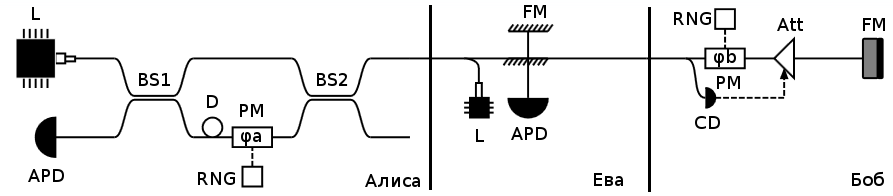
\includegraphics[width=1\linewidth]{scheme}\note{Принципиальная схема протокола показана на слайде. Суть протокола сводится к разведению частей состояния в пространстве-времени так, что по отдельности они не несут никакой полезной информации.
 Для того, чтобы получить информацию о ключе, эти части нужно свести вместе в одну точку пространства Минковского, на что требуется конечное время.}}
   \only<2>{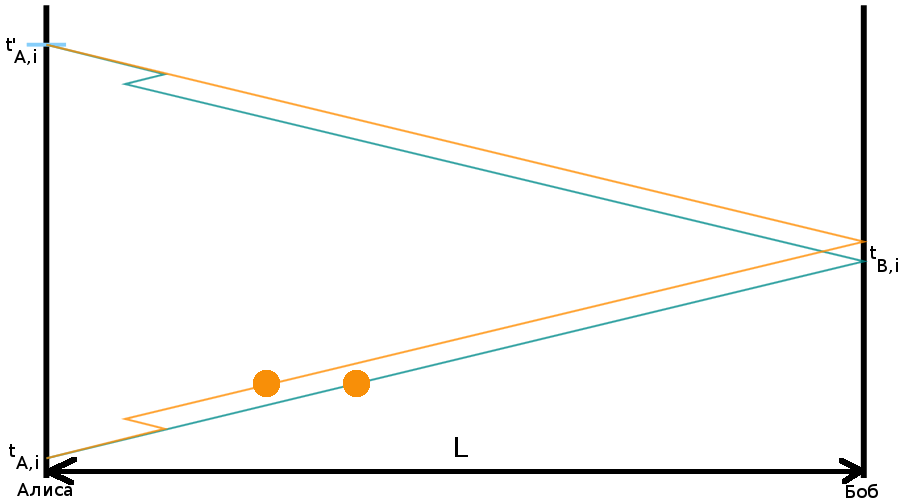
\includegraphics[width=1\linewidth]{not_catched}\note{ Алиса (слева) включает свой детектор только в определенные временные промежутки, когда, по ее расчетам, должно прийти ответное состояние.}}
   \only<3>{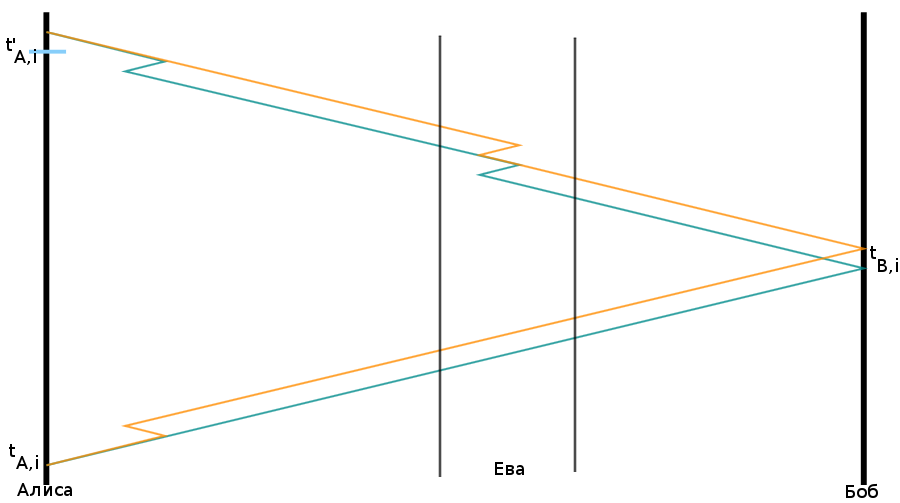
\includegraphics[width=1\linewidth]{eve_detected}\note{ Если в канале передачи присутствует злоумышленник, то он потратит некоторое время сначала на сведение частей состояние вместе, получение необходимой ему информации, а затем на разведение частей обратно.
 В результате состояние придет к Алисе с задержкой, которая будет задетектирована.}}
 \end{frame}

 
 
\section{Исследование каскадного протокола коррекции ошибок}
 \begin{frame}{Каскадный метод коррекции ошибок}
    \only<1>{В канале связи (в частности если это открытое пространство) неизбежно присутствуют помехи, вносящие ошибки в ключ. Их необходимо исправить, выдав как можно меньше информации о ключе возможному подслушивателю. \note{После проведения квантовой части протокола, требуется коррекция ошибок в силу наличия помех в канале связи.
 Коррекция ошибок производится по аутентичному каналу, то есть который можно свободно прослушивать, но невозможно изменить передаваемые по нему данные (газеты, twitter итд).}}
   \only<2>{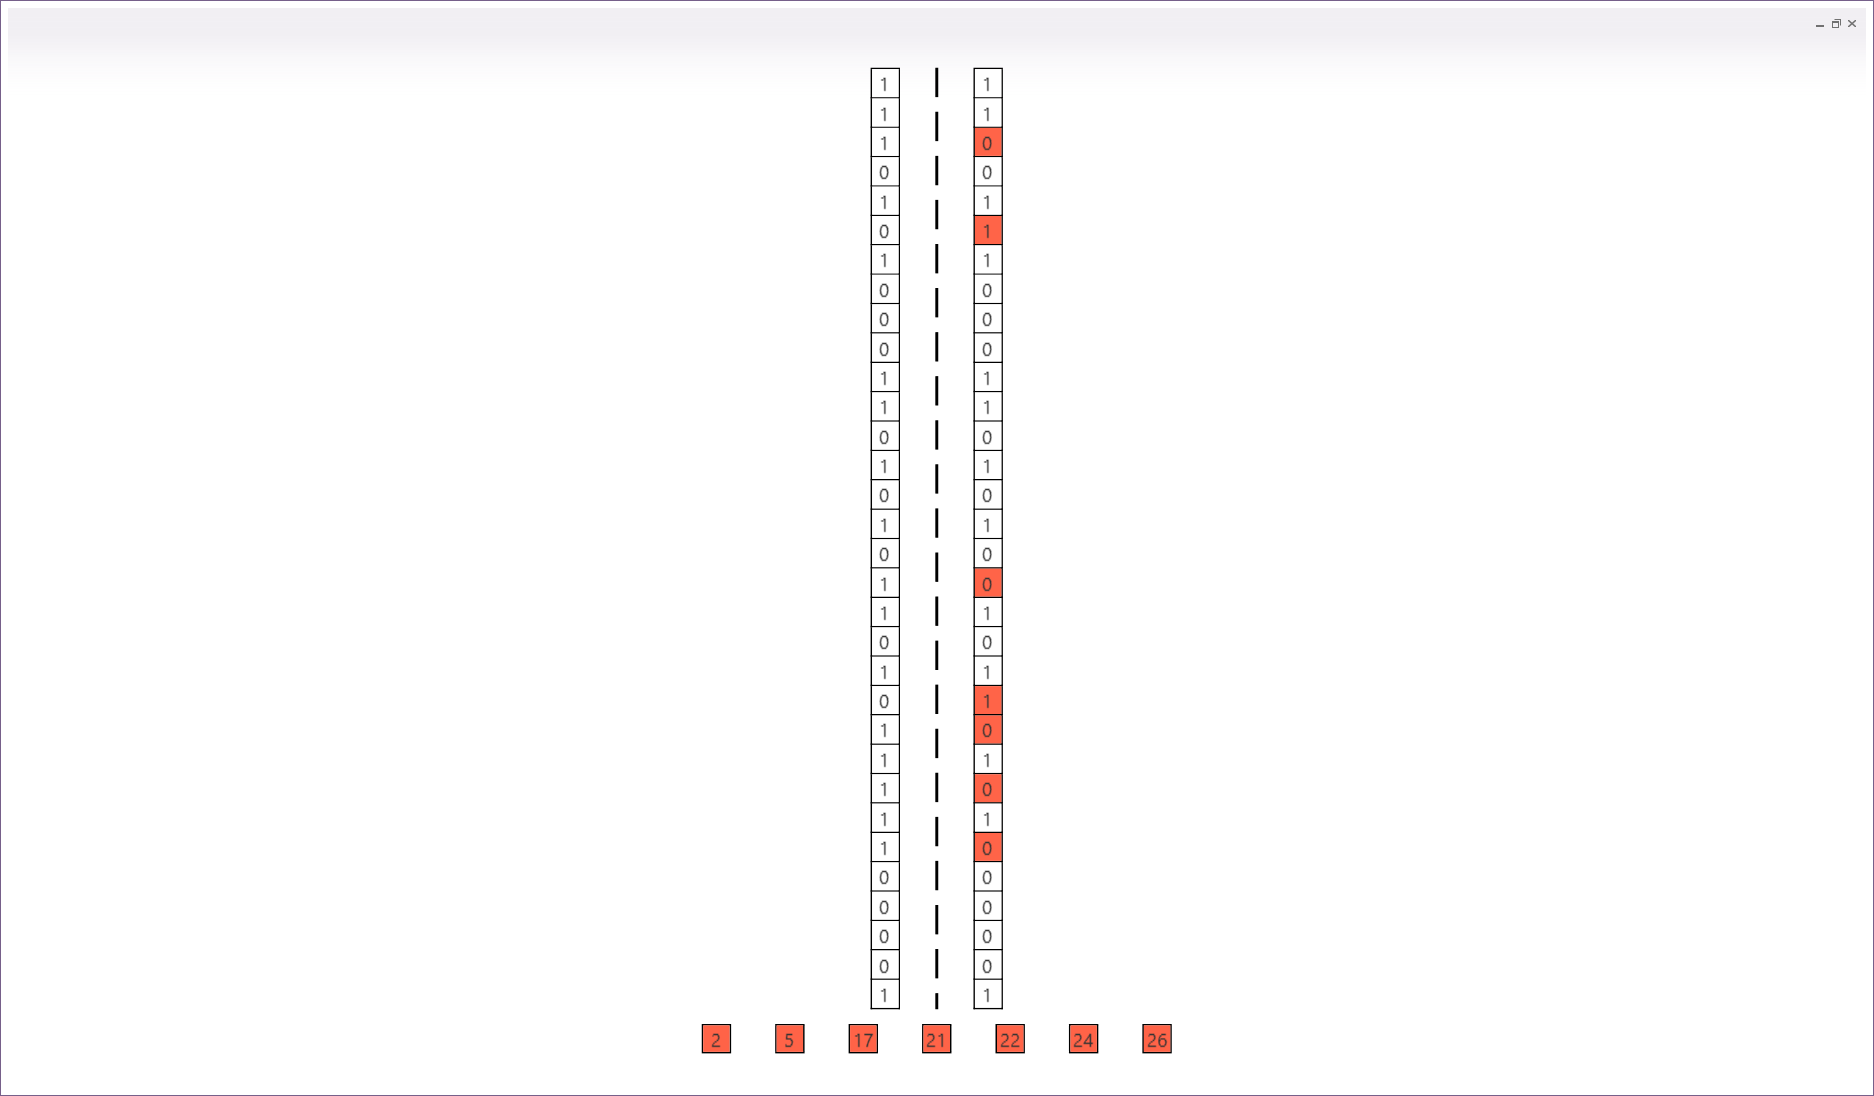
\includegraphics[width=1\linewidth]{chapter3/cascade_screenshots/01_start_state}}
   \only<3>{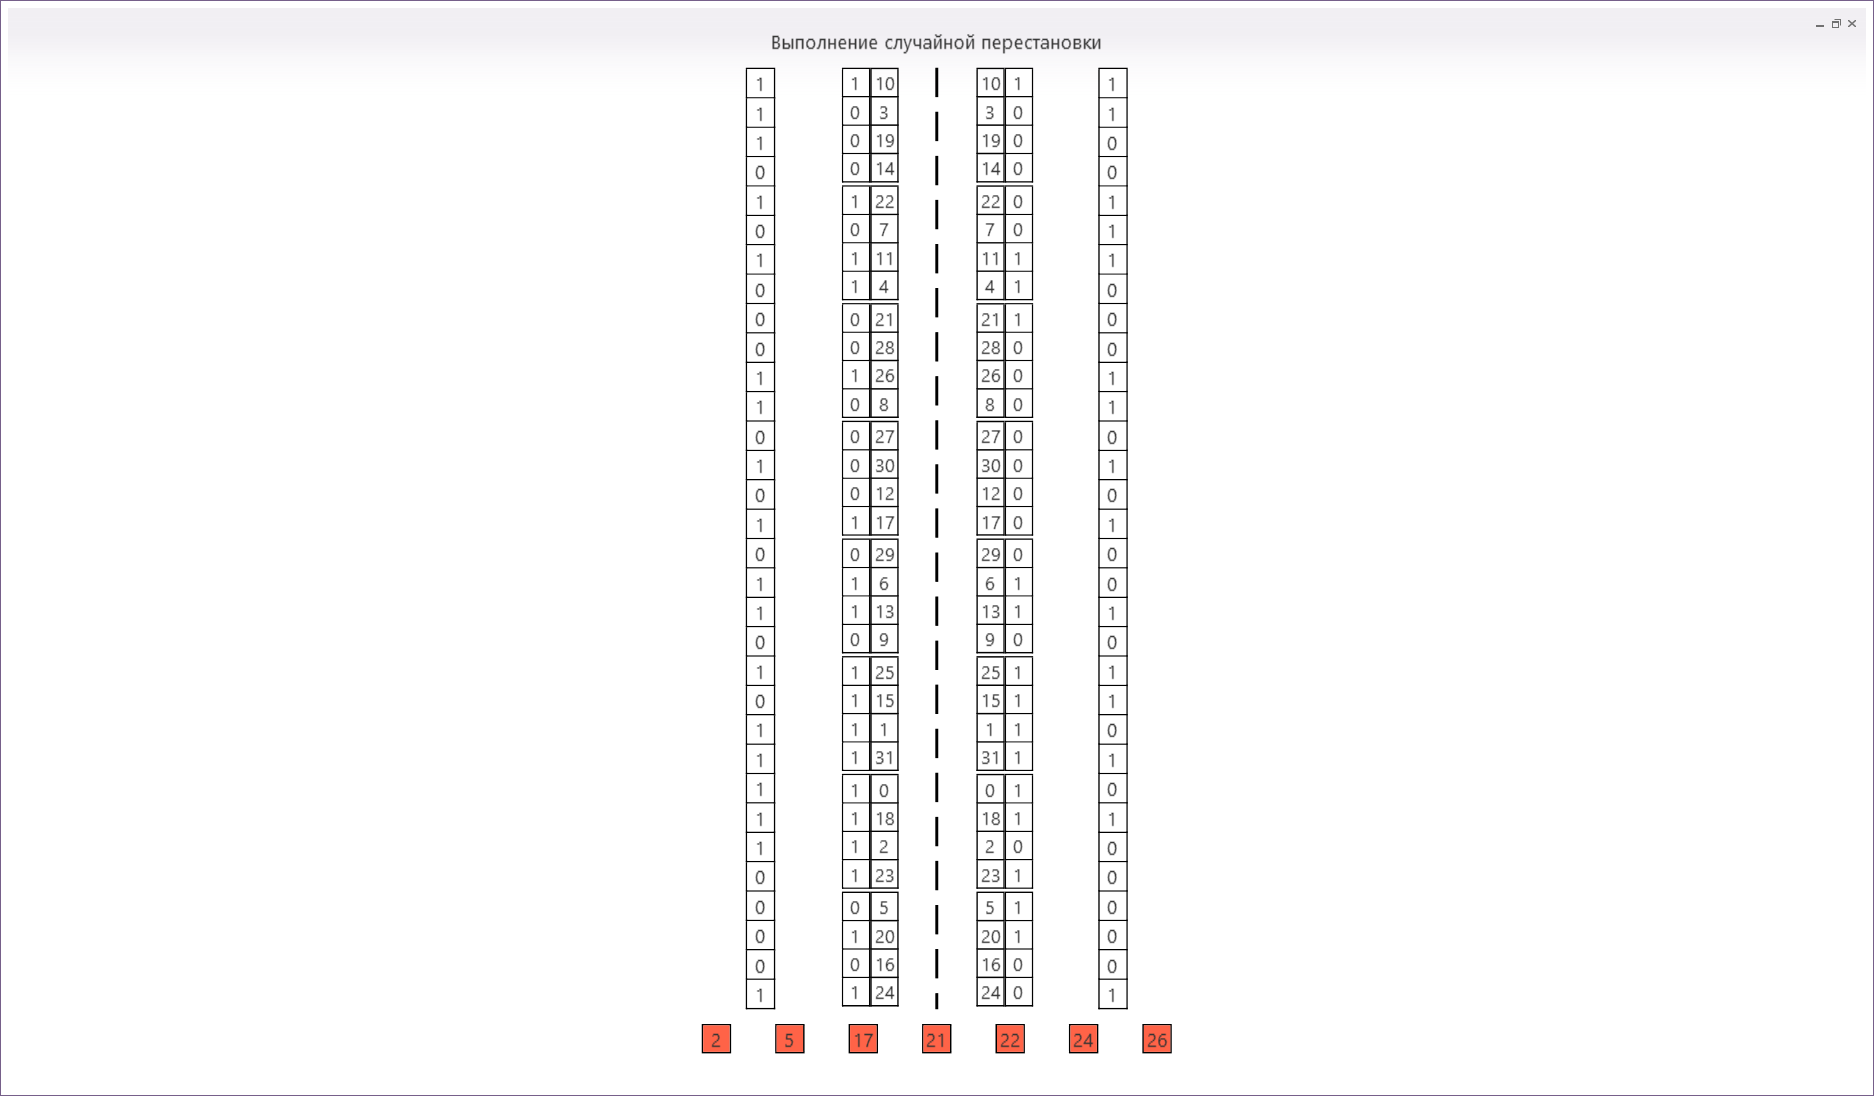
\includegraphics[width=1\linewidth]{chapter3/cascade_screenshots/02_fill_blocks}}
   \only<4>{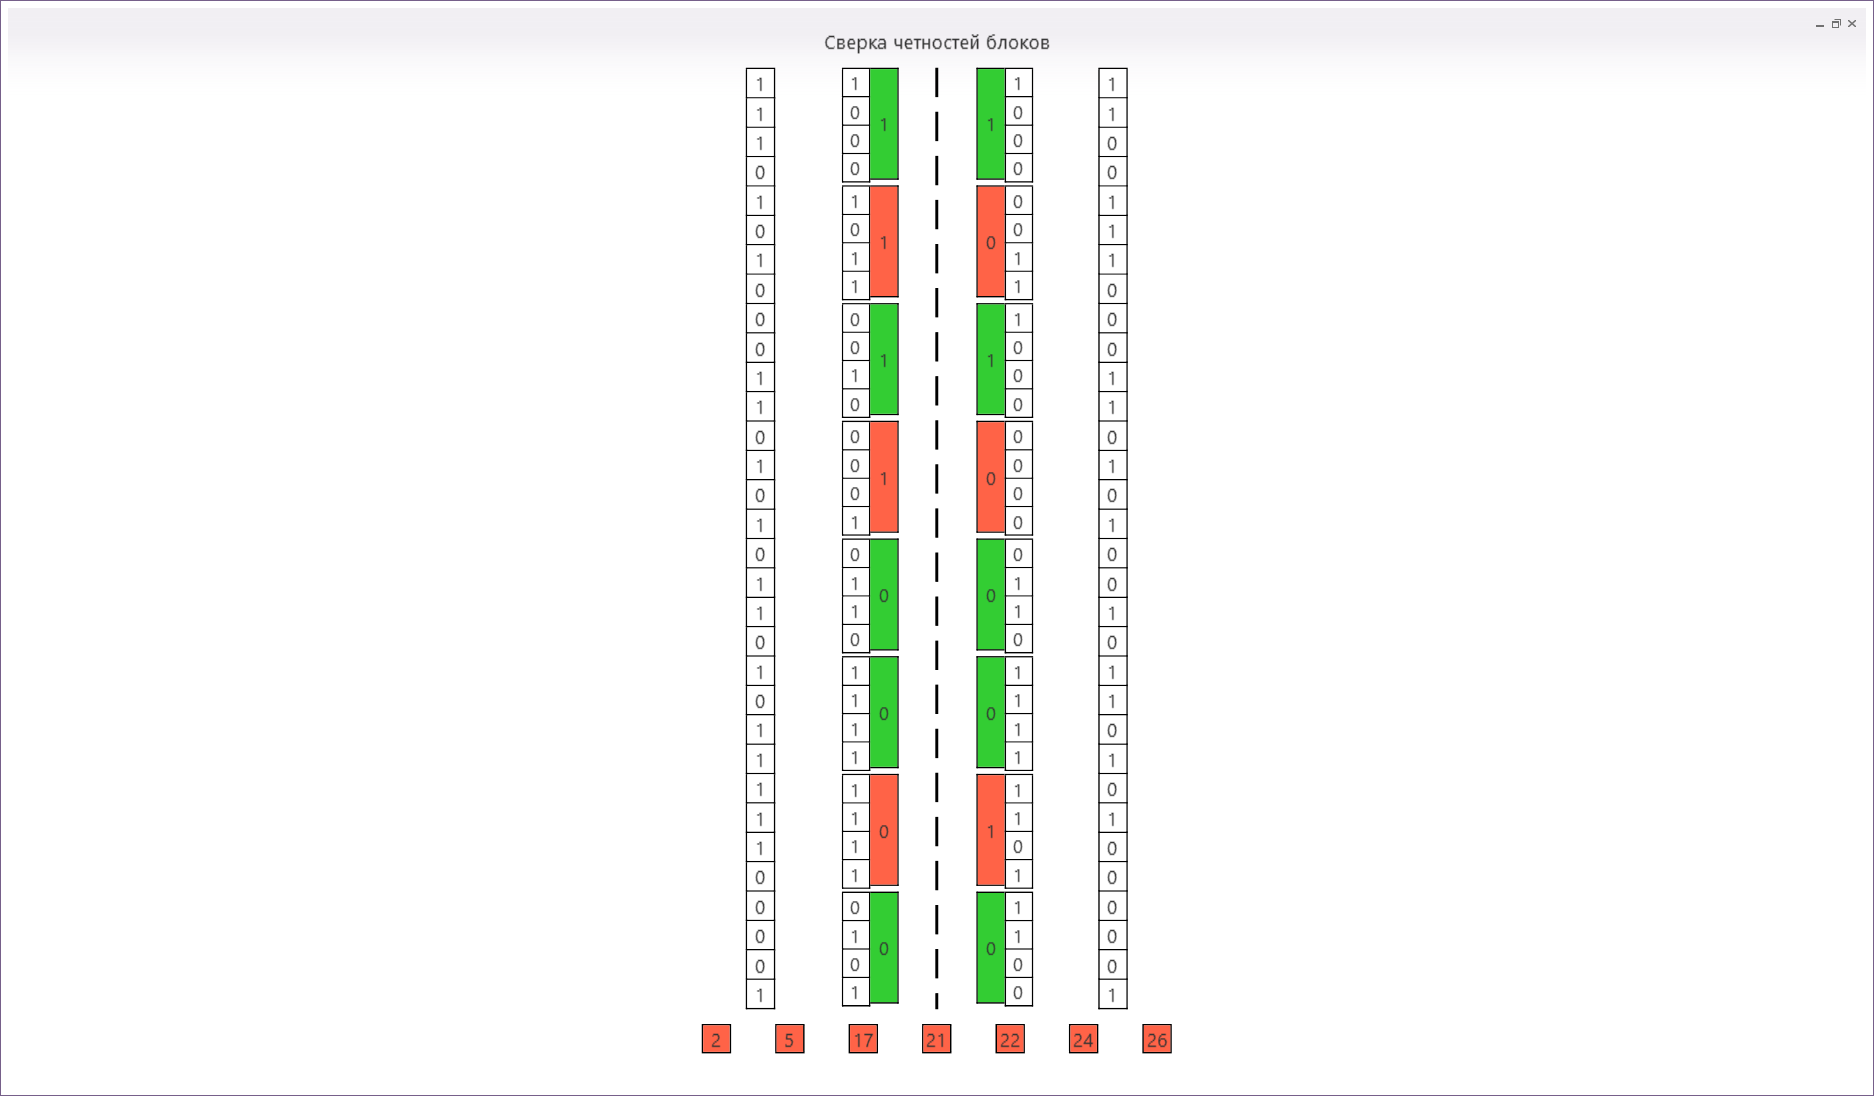
\includegraphics[width=1\linewidth]{chapter3/cascade_screenshots/03_check_parities}}
   \only<5>{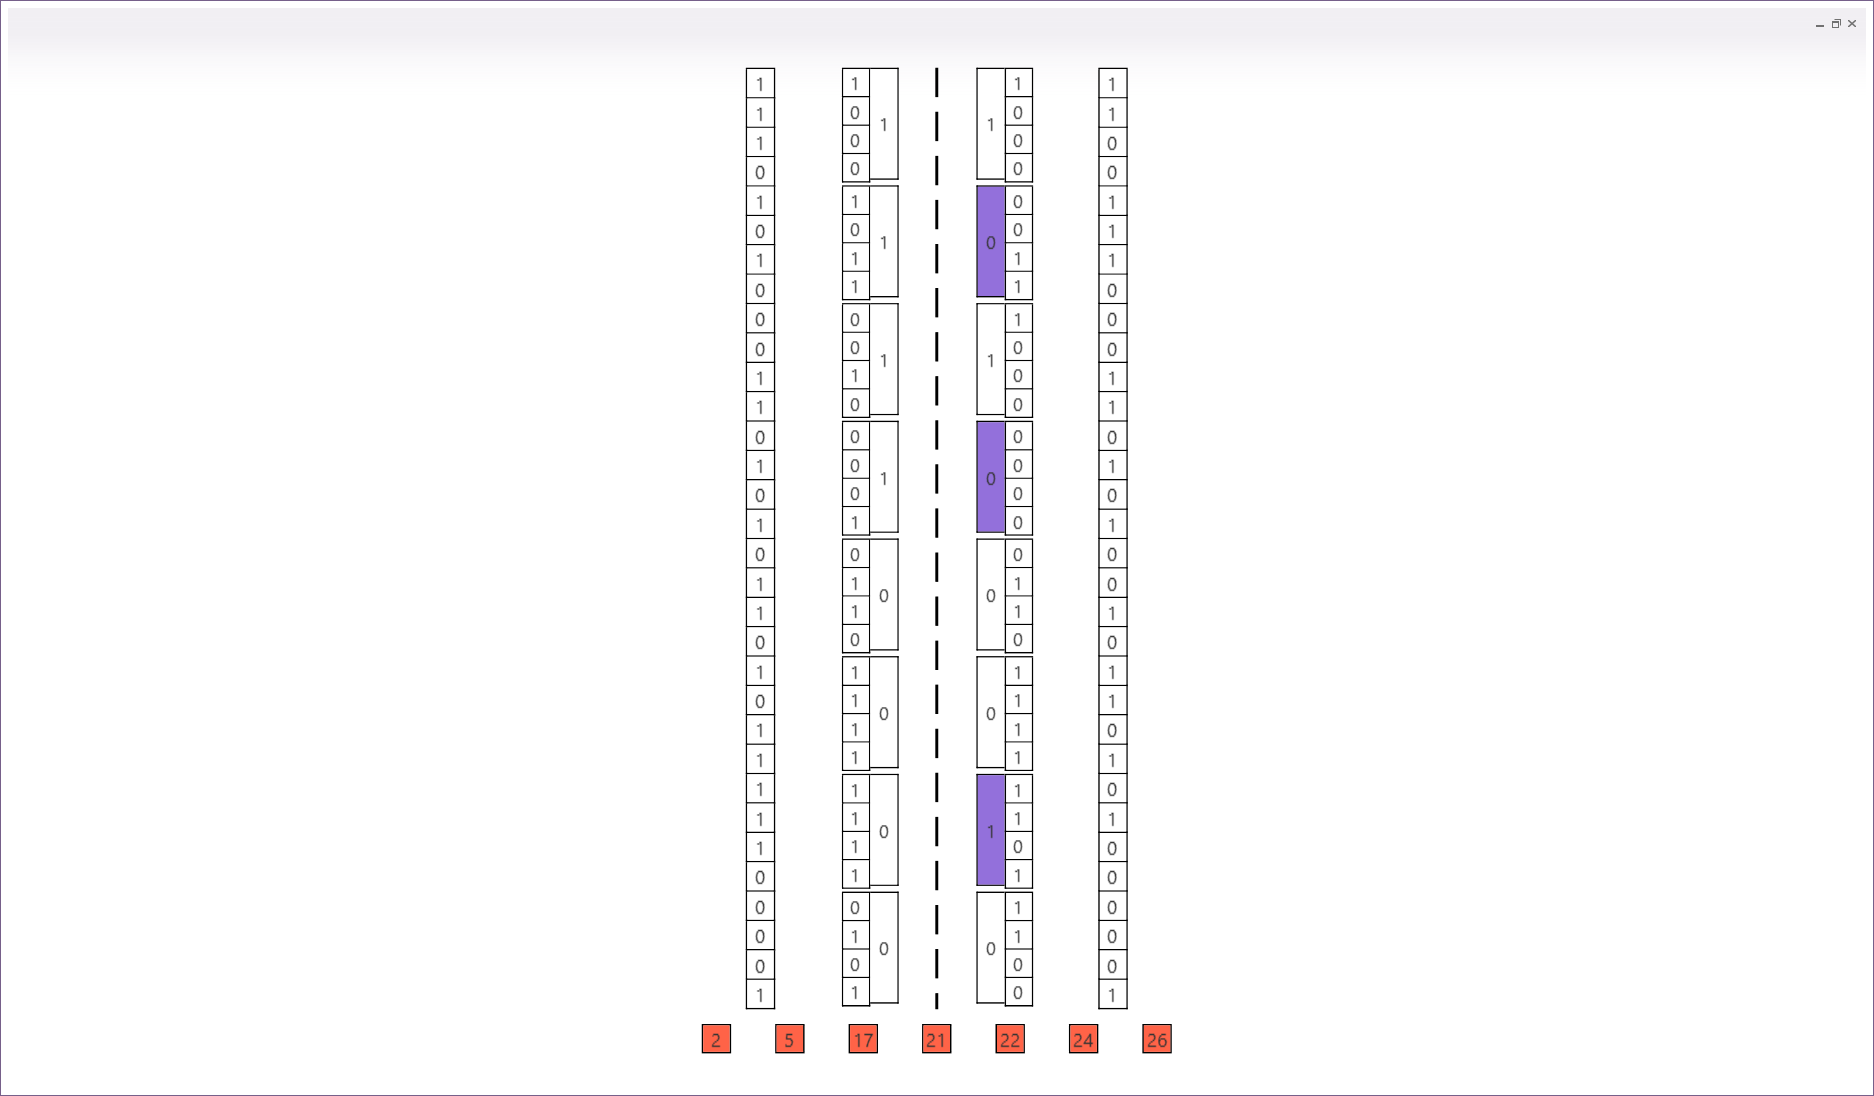
\includegraphics[width=1\linewidth]{chapter3/cascade_screenshots/04_set_odd_errors}}
   \only<6>{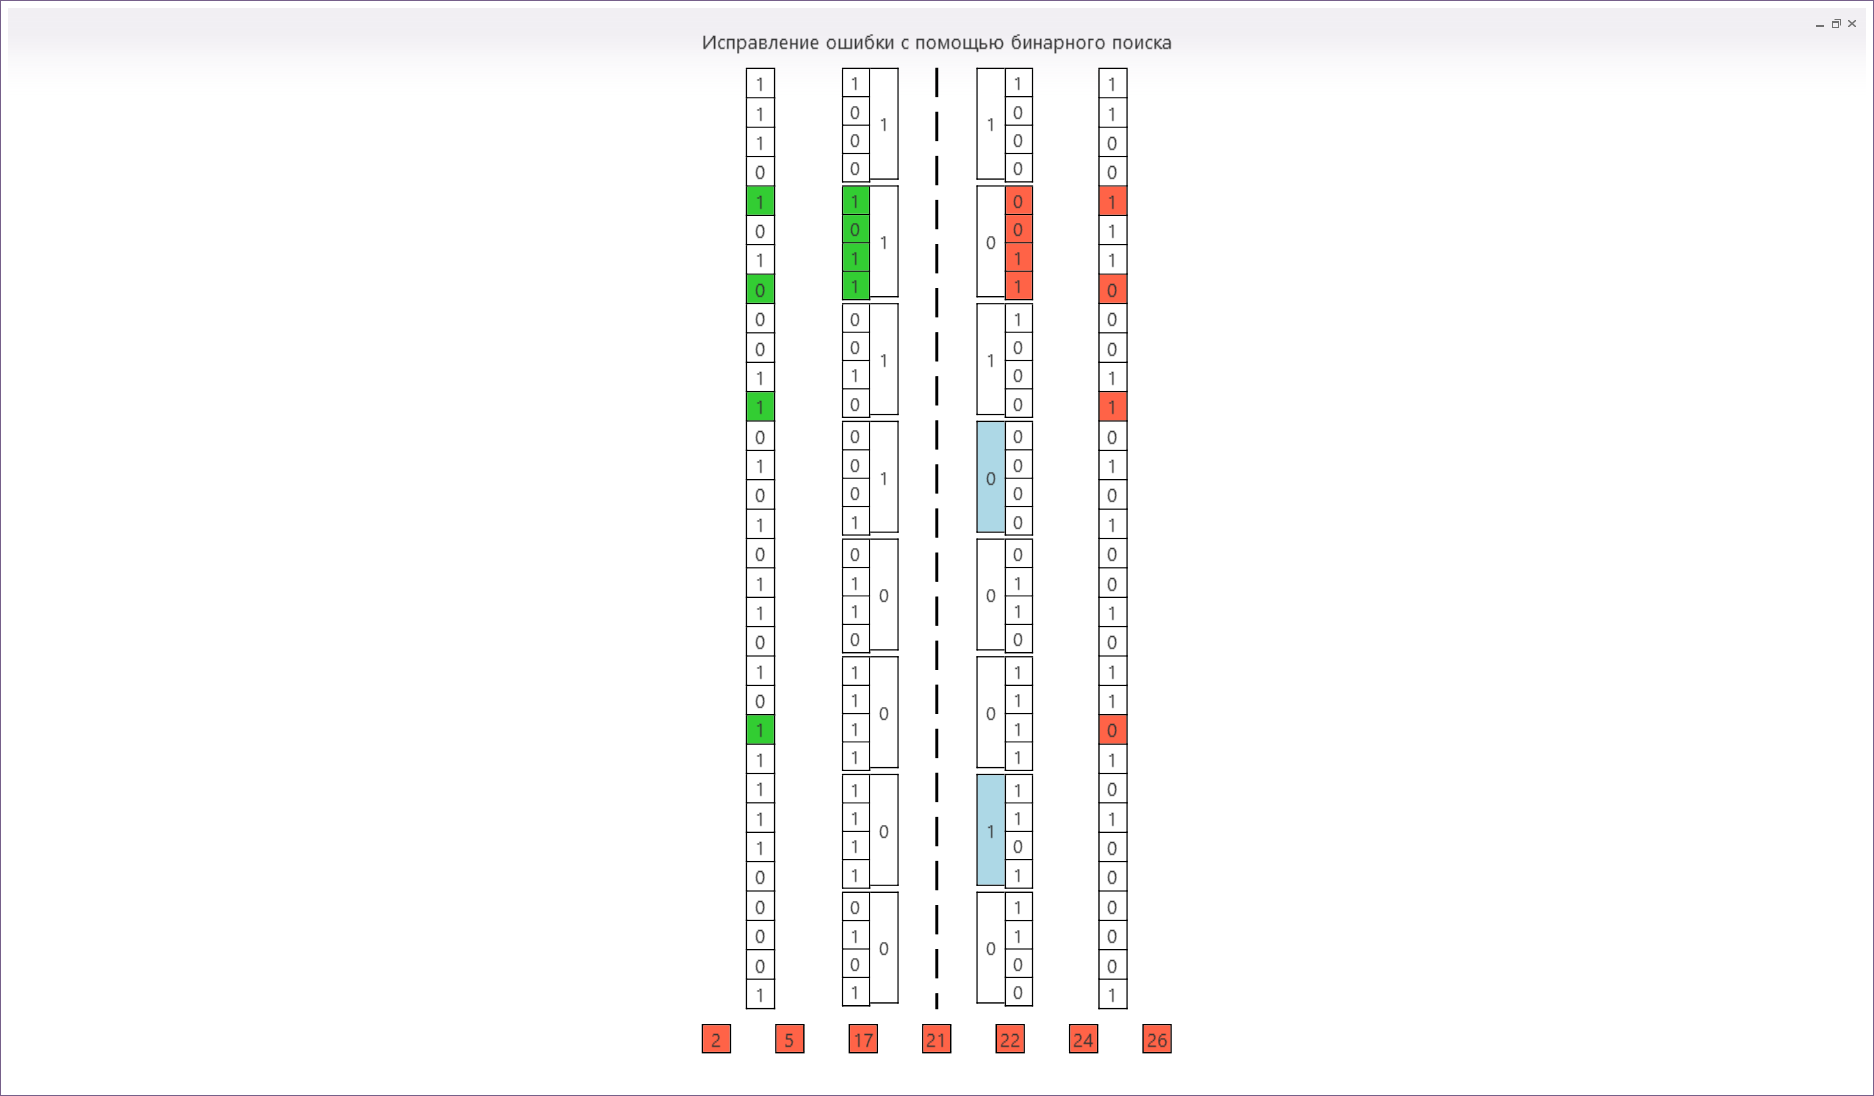
\includegraphics[width=1\linewidth]{chapter3/cascade_screenshots/05_binary}}
   \only<7>{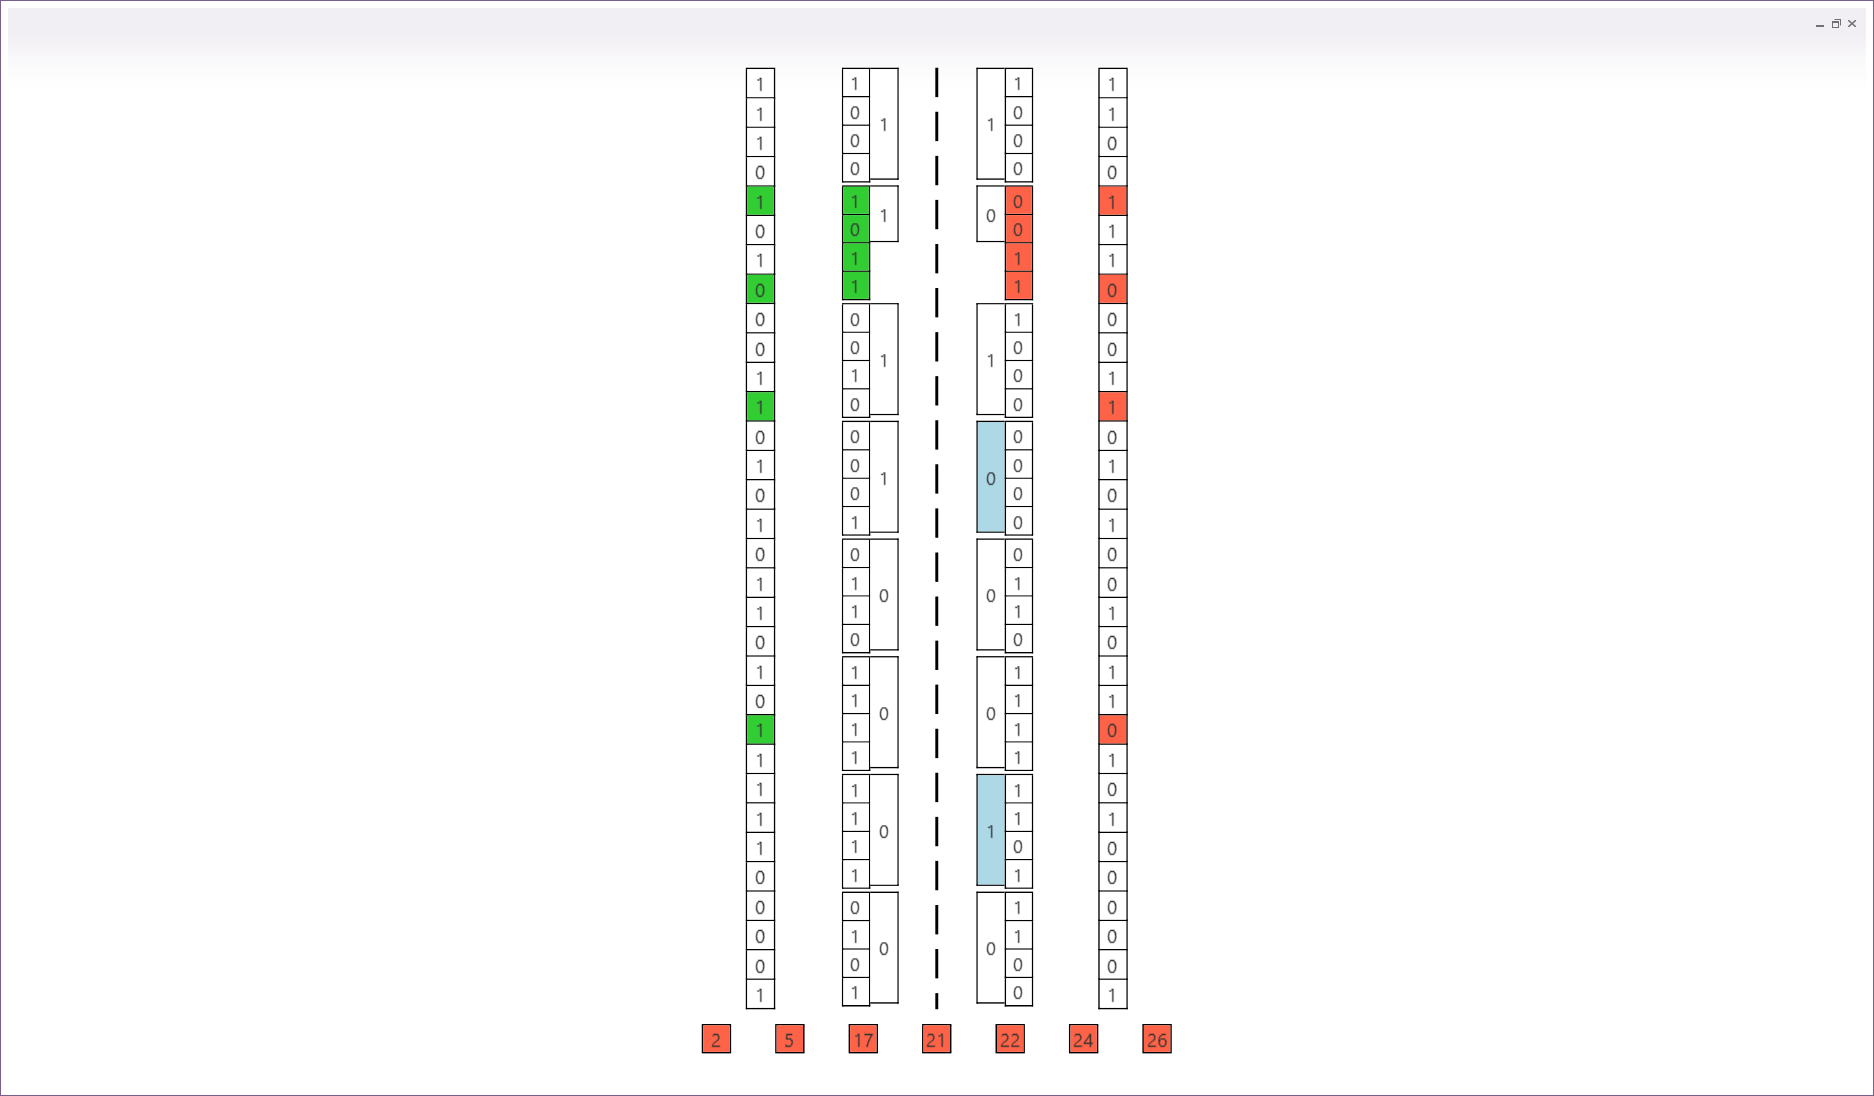
\includegraphics[width=1\linewidth]{chapter3/cascade_screenshots/06_binary}}
   \only<8>{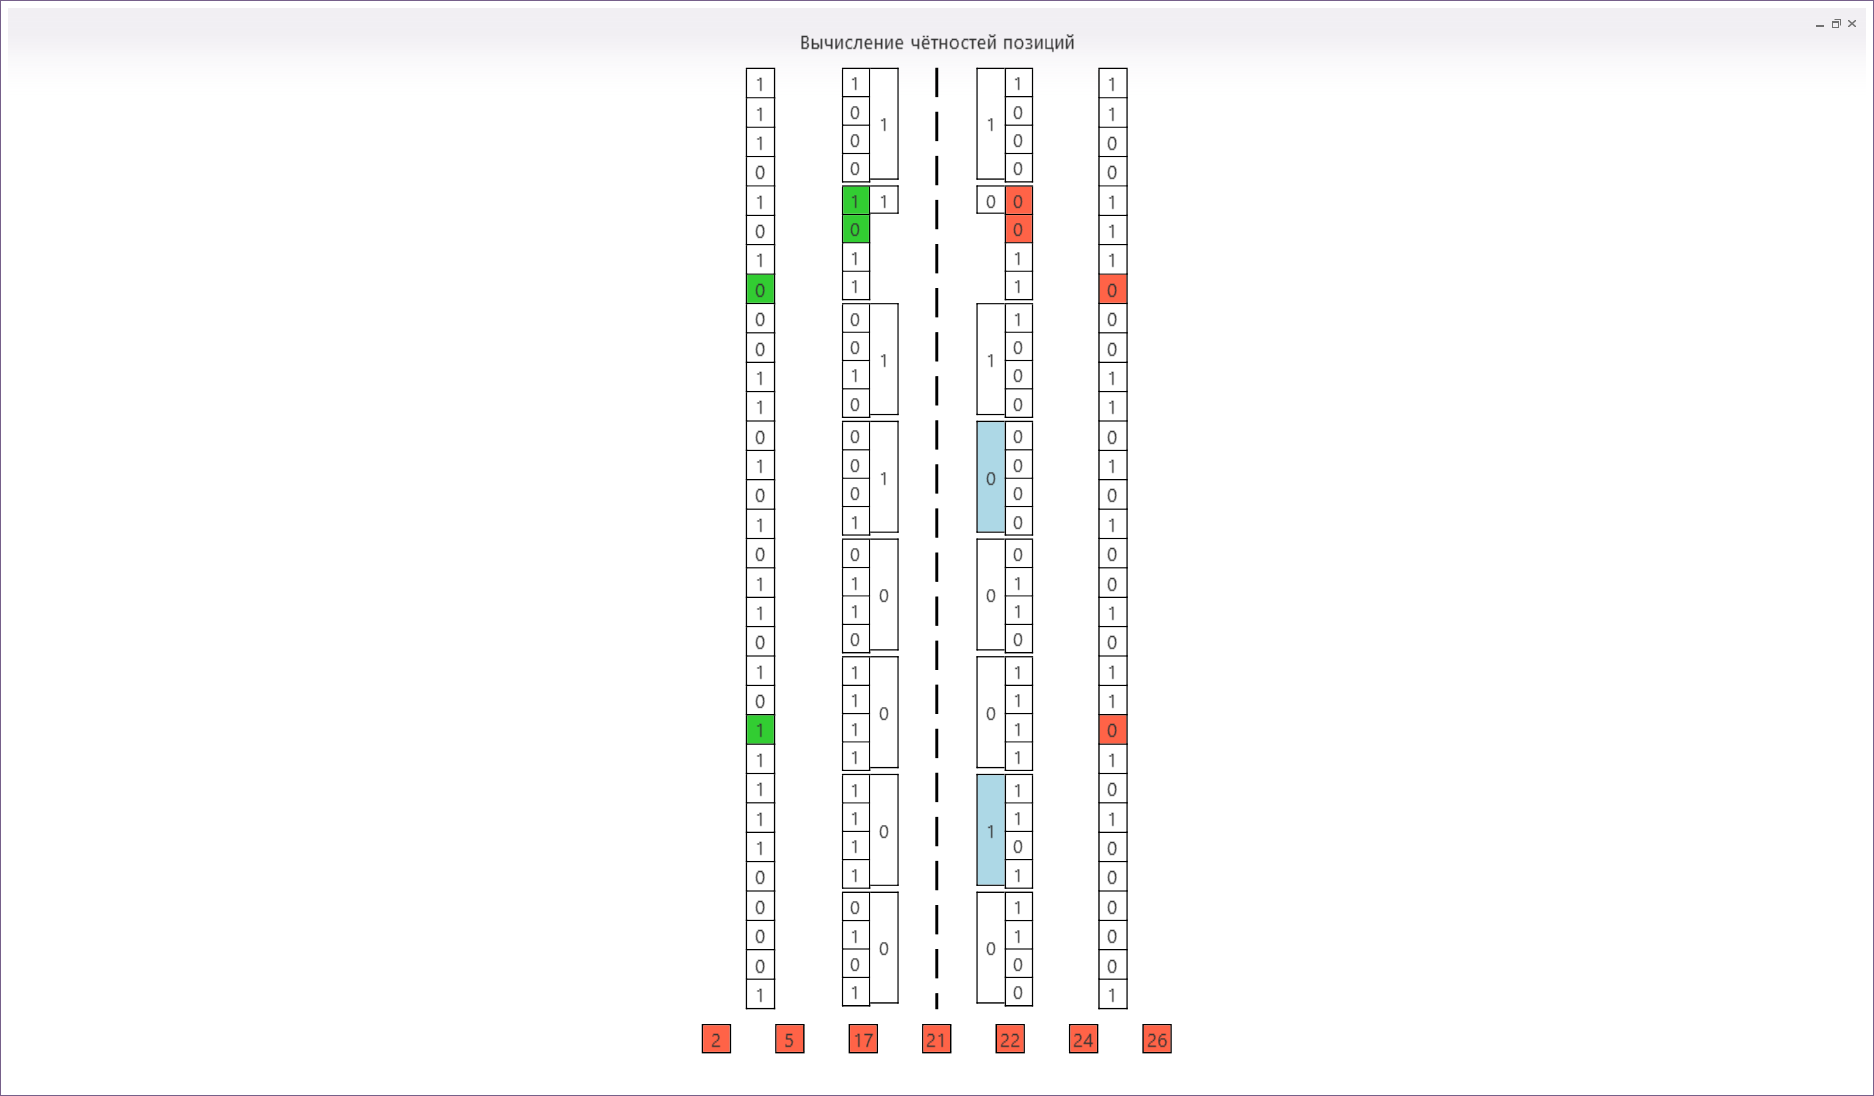
\includegraphics[width=1\linewidth]{chapter3/cascade_screenshots/07_binary}}
   \only<9>{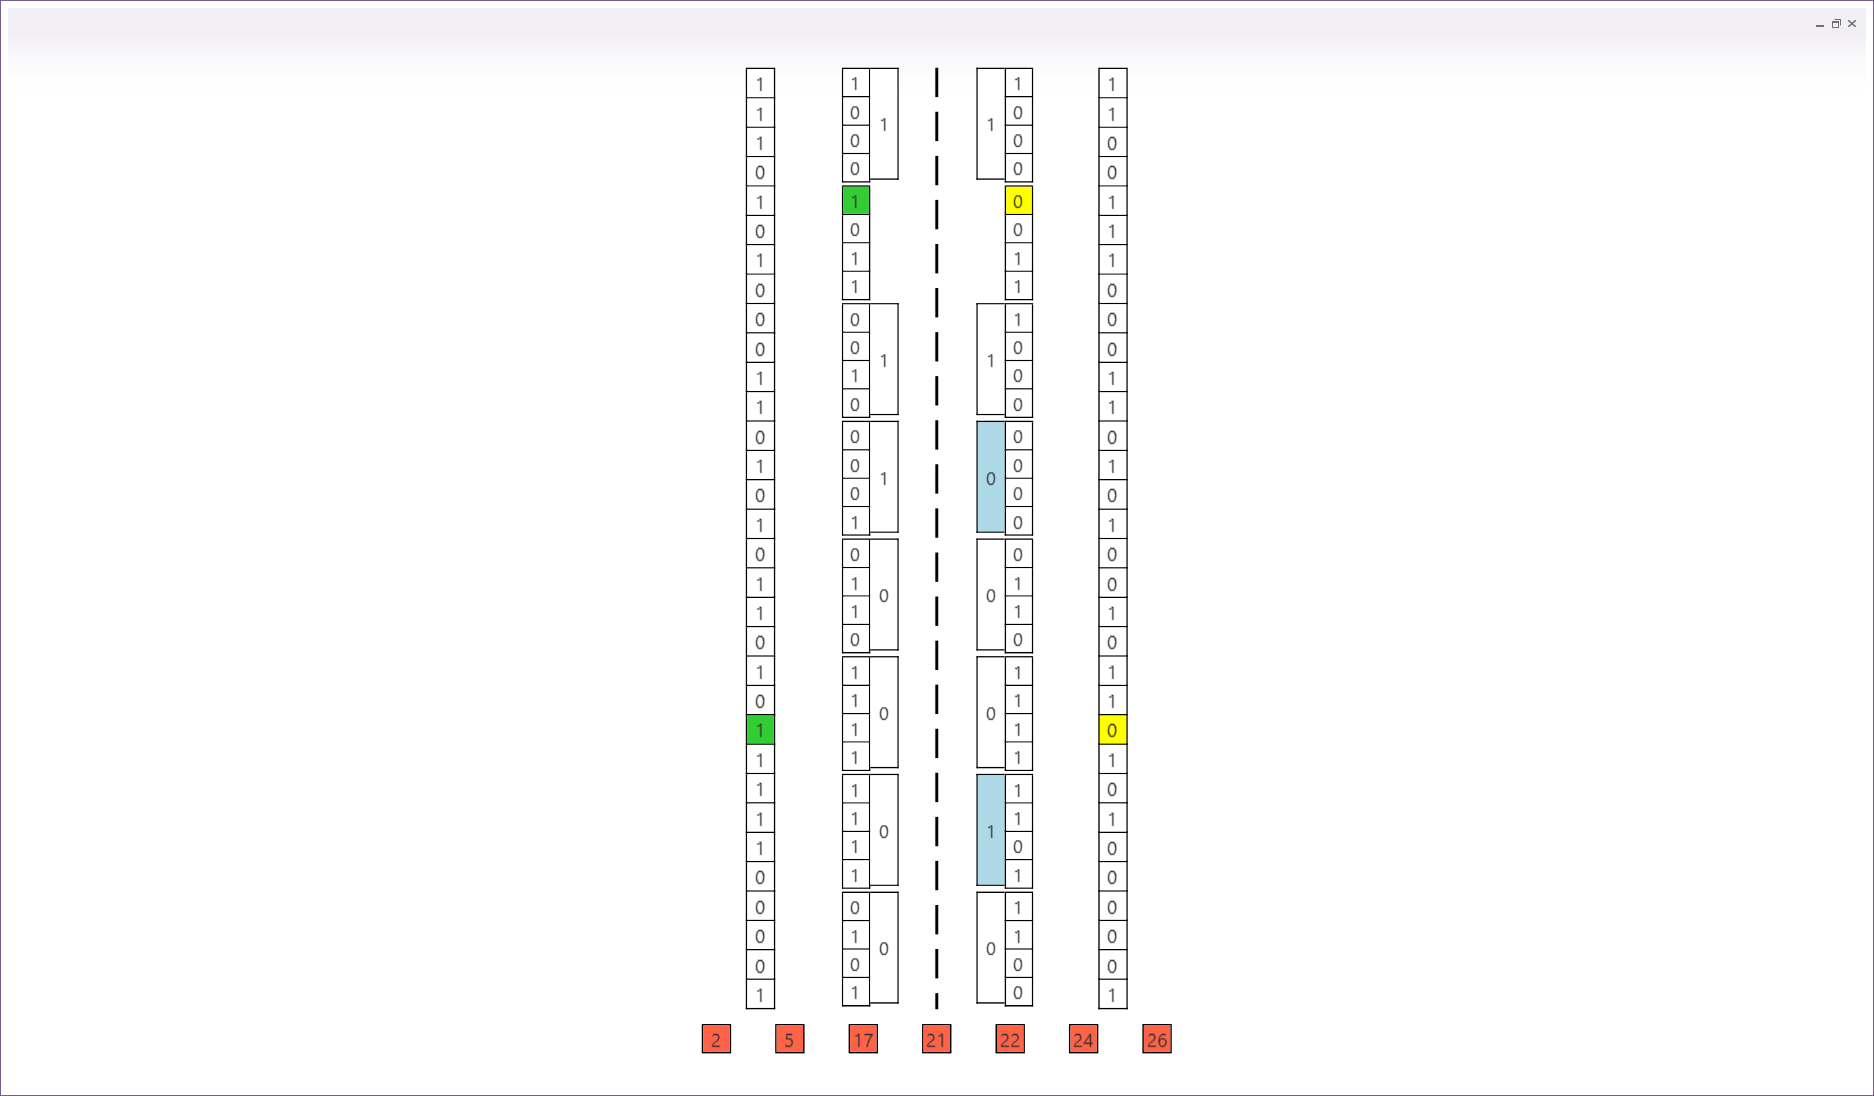
\includegraphics[width=1\linewidth]{chapter3/cascade_screenshots/08_found_error}}
   \only<10>{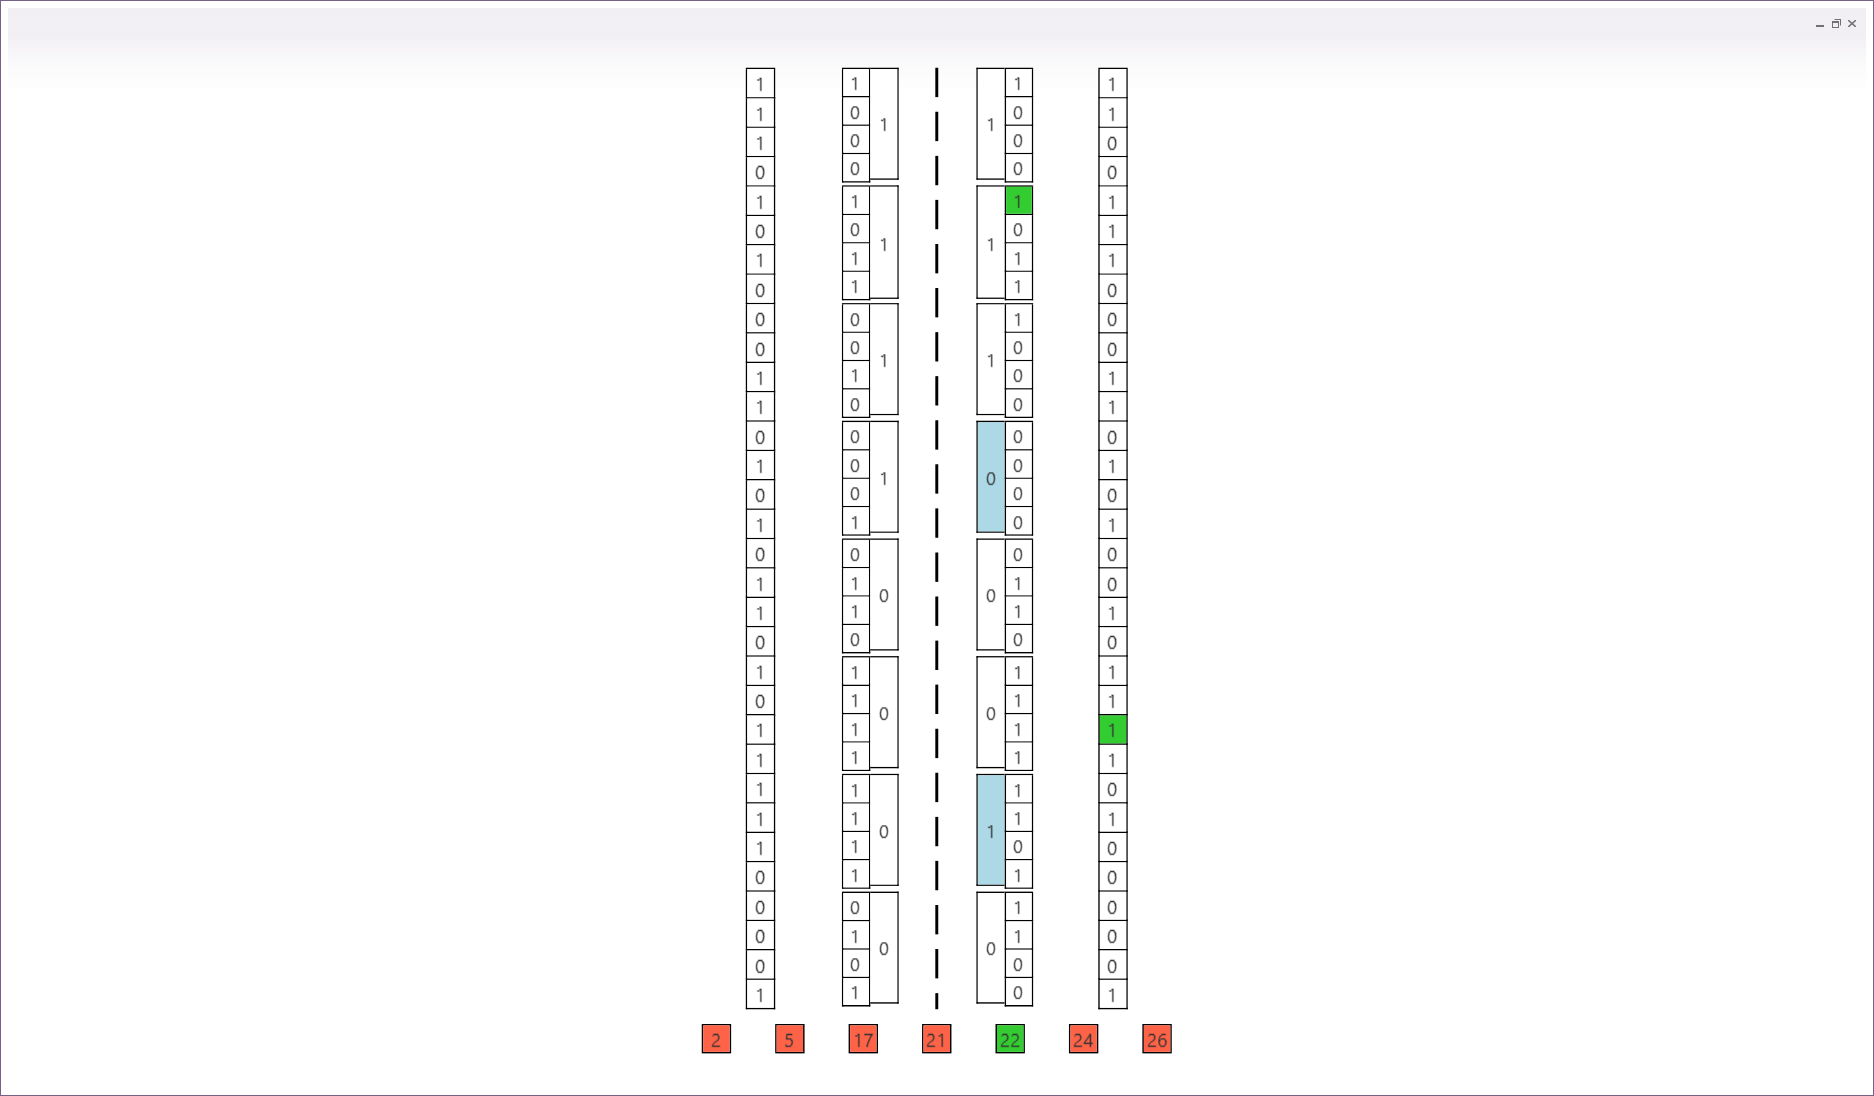
\includegraphics[width=1\linewidth]{chapter3/cascade_screenshots/09_error_corrected}}
   \only<11>{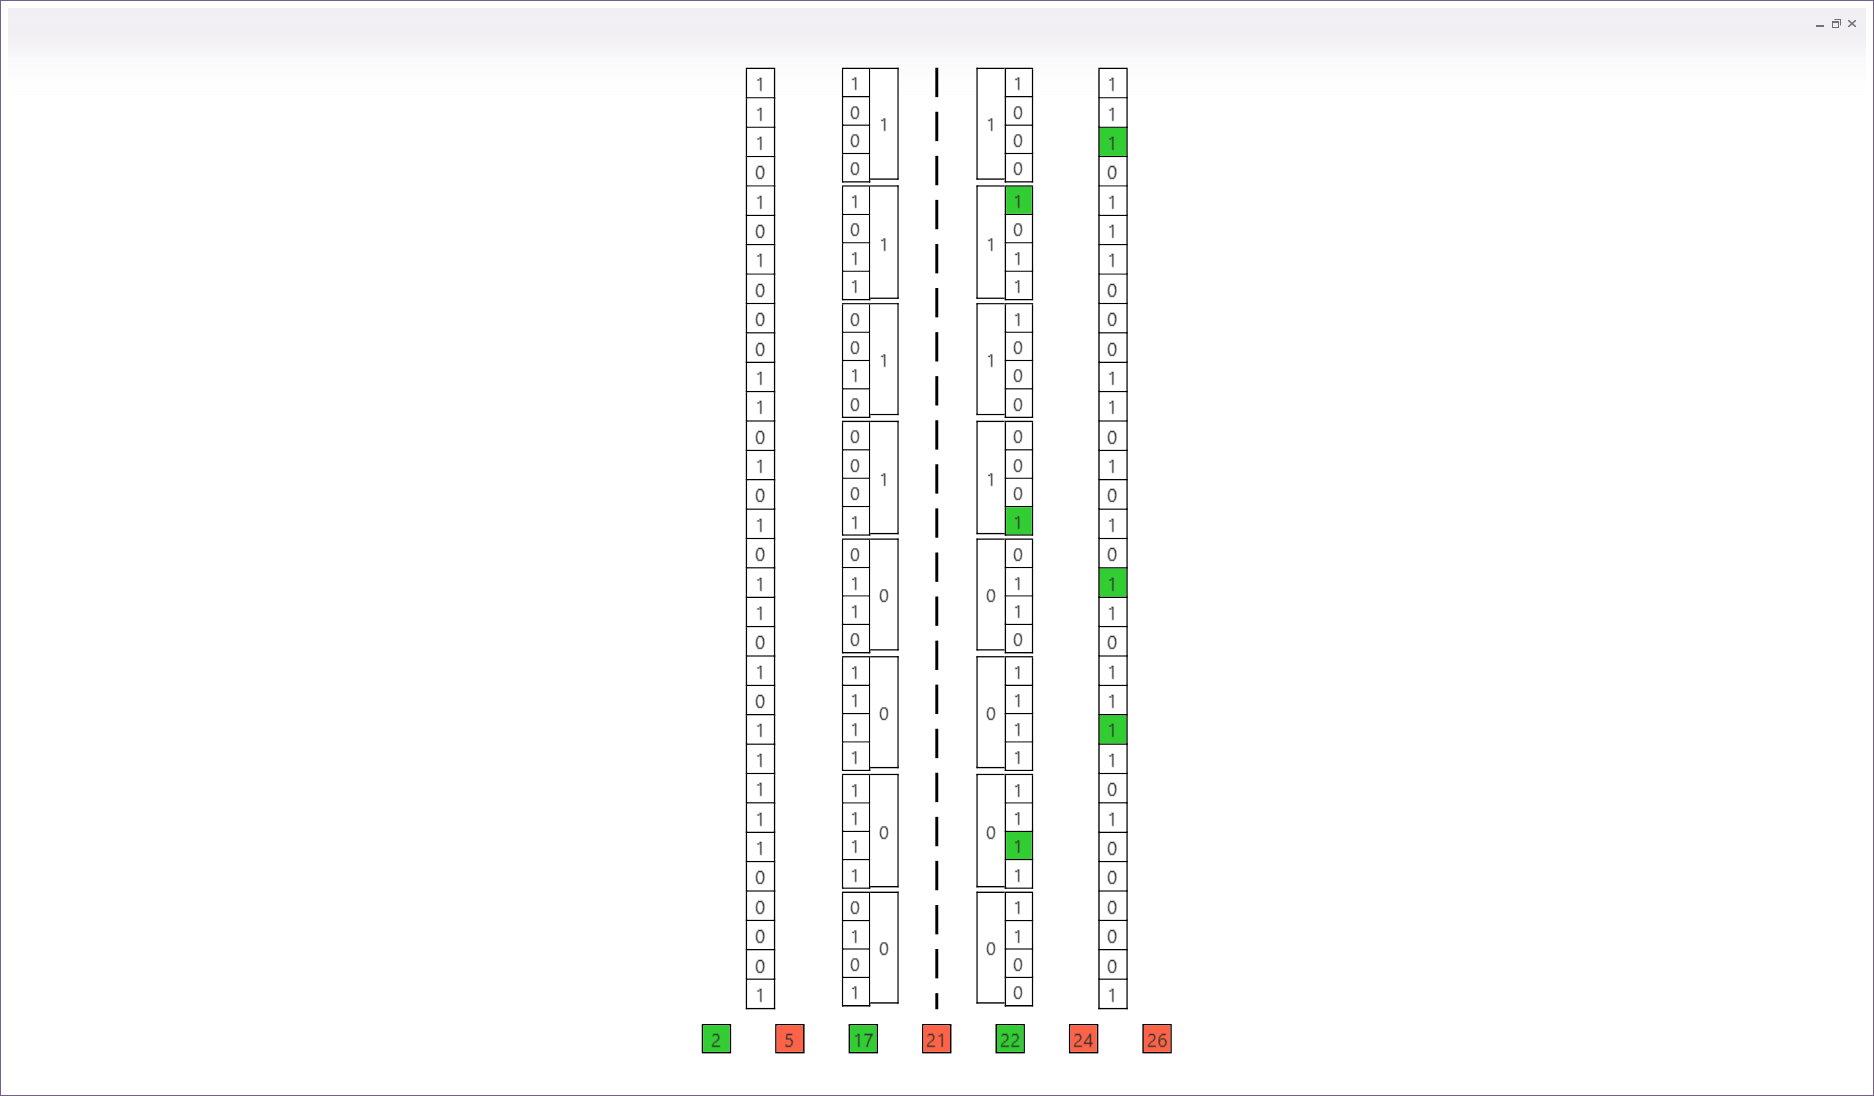
\includegraphics[width=1\linewidth]{chapter3/cascade_screenshots/10_pass_complete}}
   \only<12>{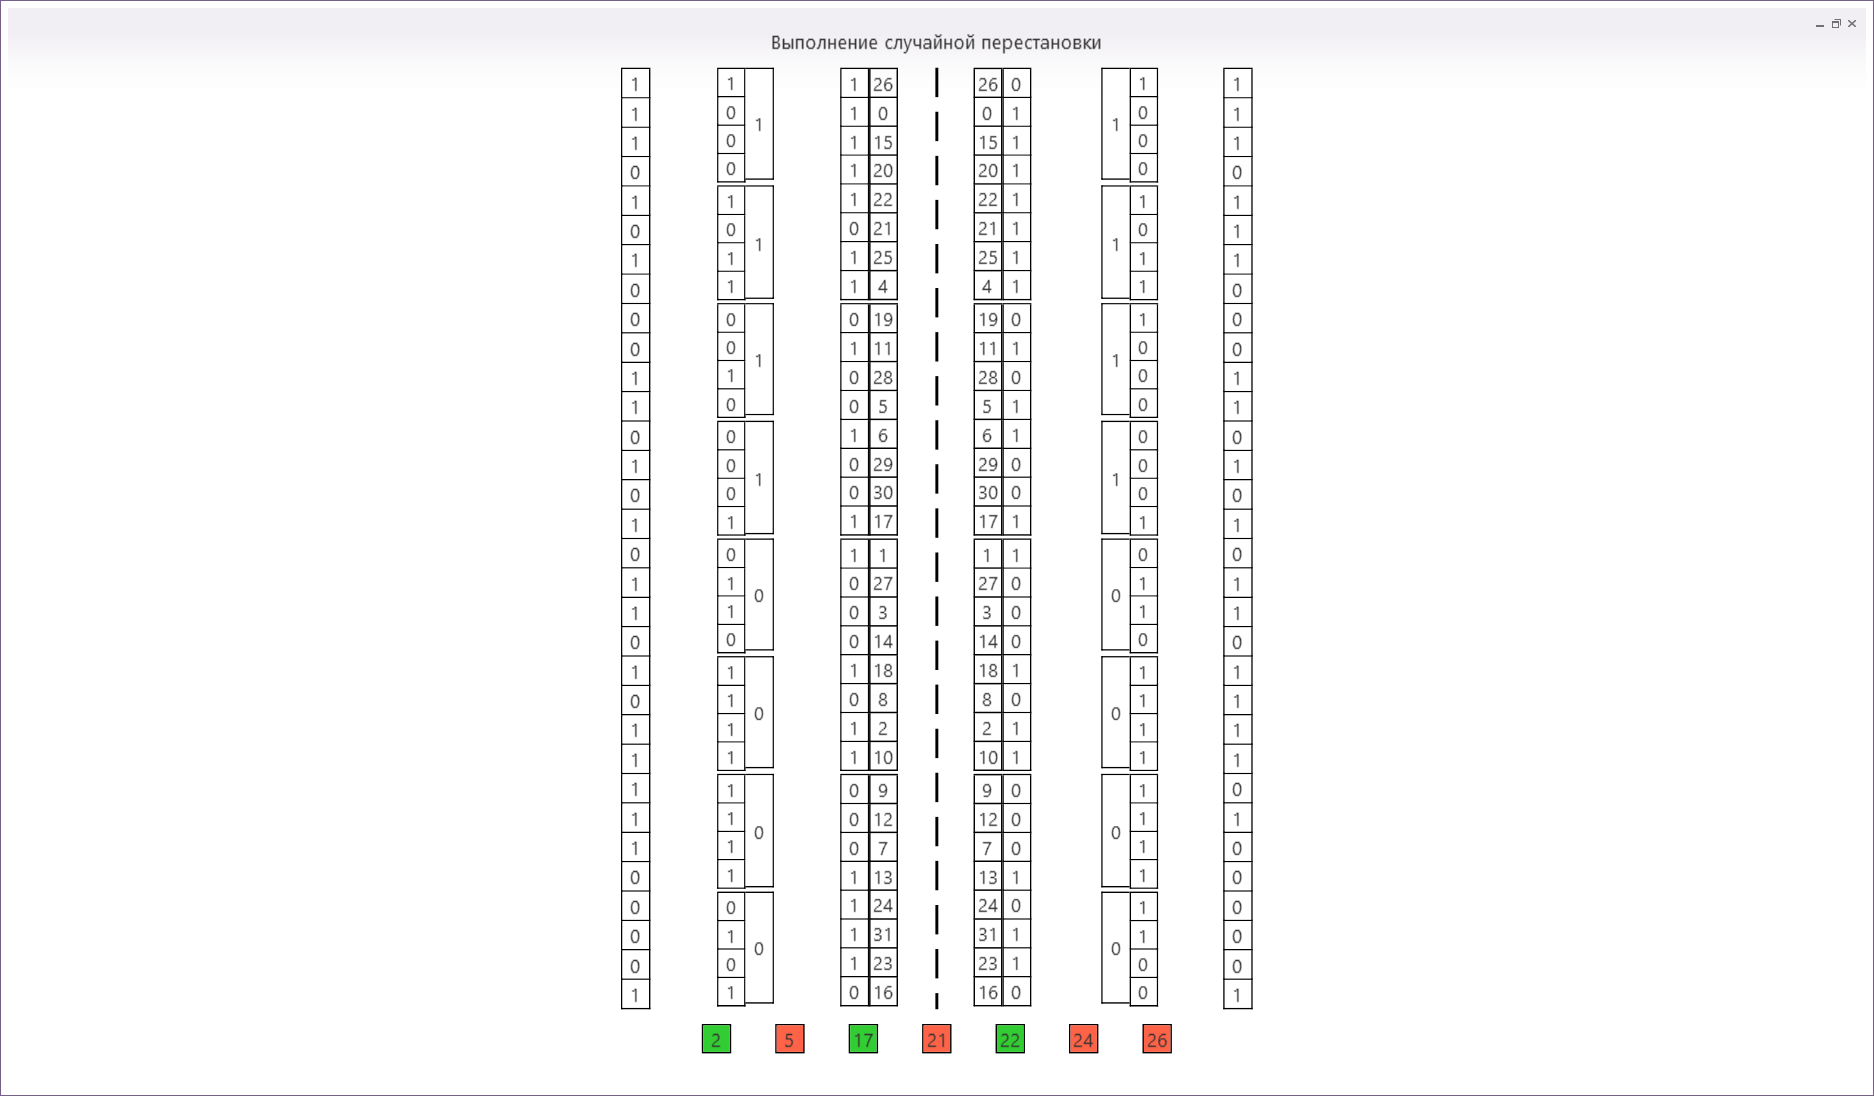
\includegraphics[width=1\linewidth]{chapter3/cascade_screenshots/11_fill_blocks}}
   \only<13>{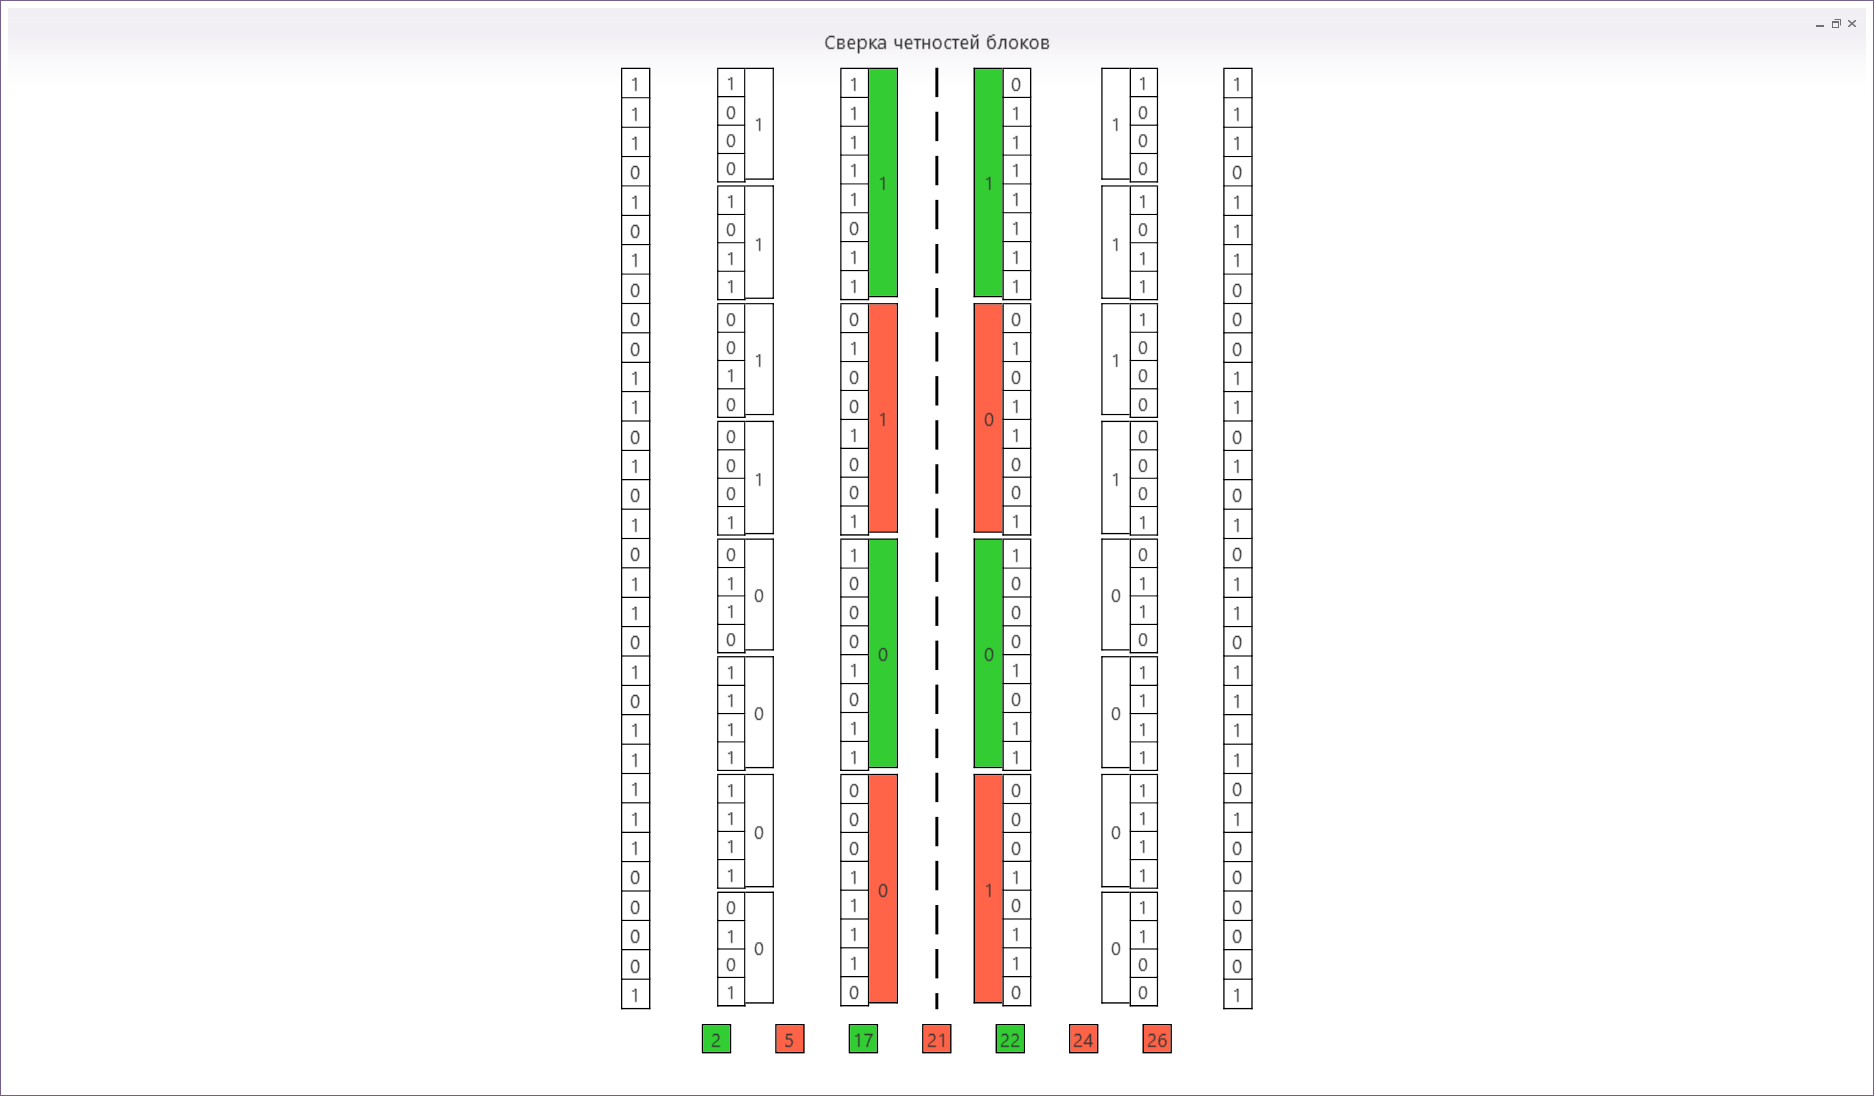
\includegraphics[width=1\linewidth]{chapter3/cascade_screenshots/12_check_parities}}
   \only<14>{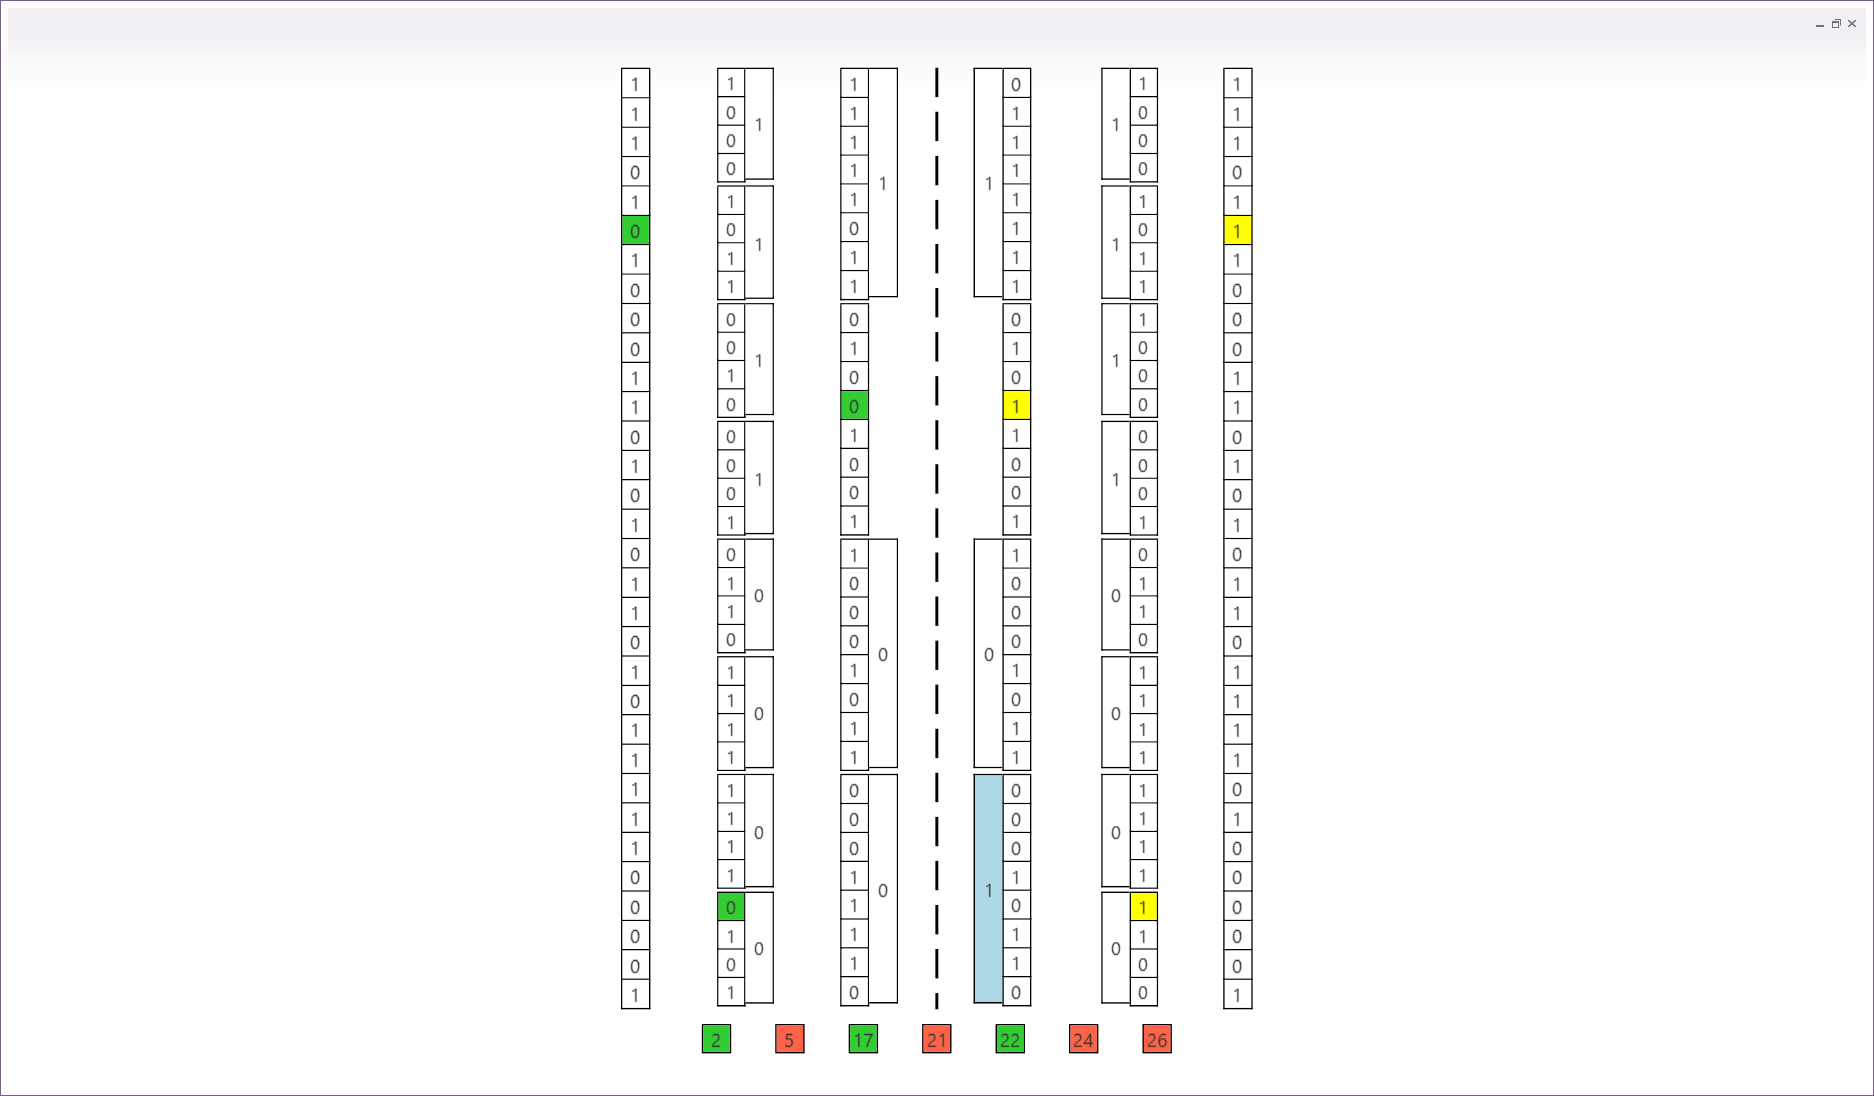
\includegraphics[width=1\linewidth]{chapter3/cascade_screenshots/13_error_found}}
   \only<15>{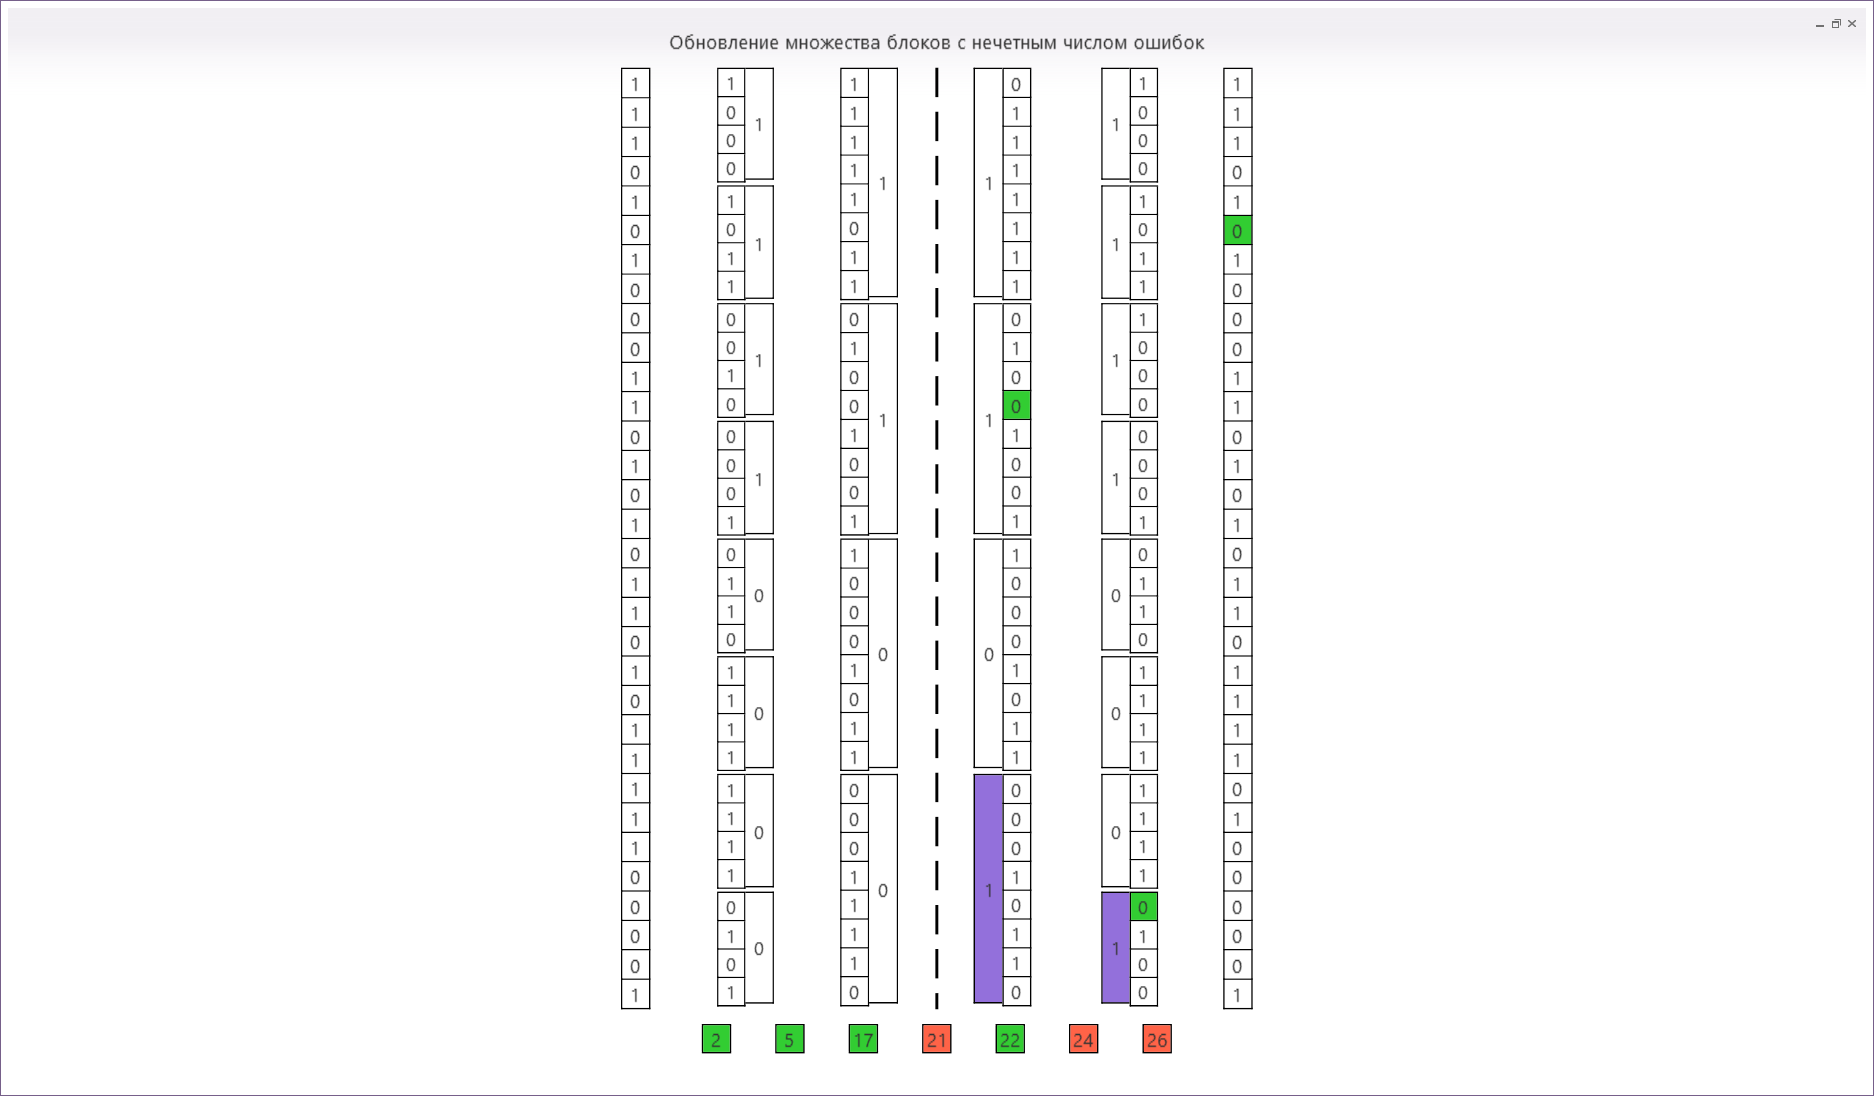
\includegraphics[width=1\linewidth]{chapter3/cascade_screenshots/14_error_backtrace}}
   \only<16>{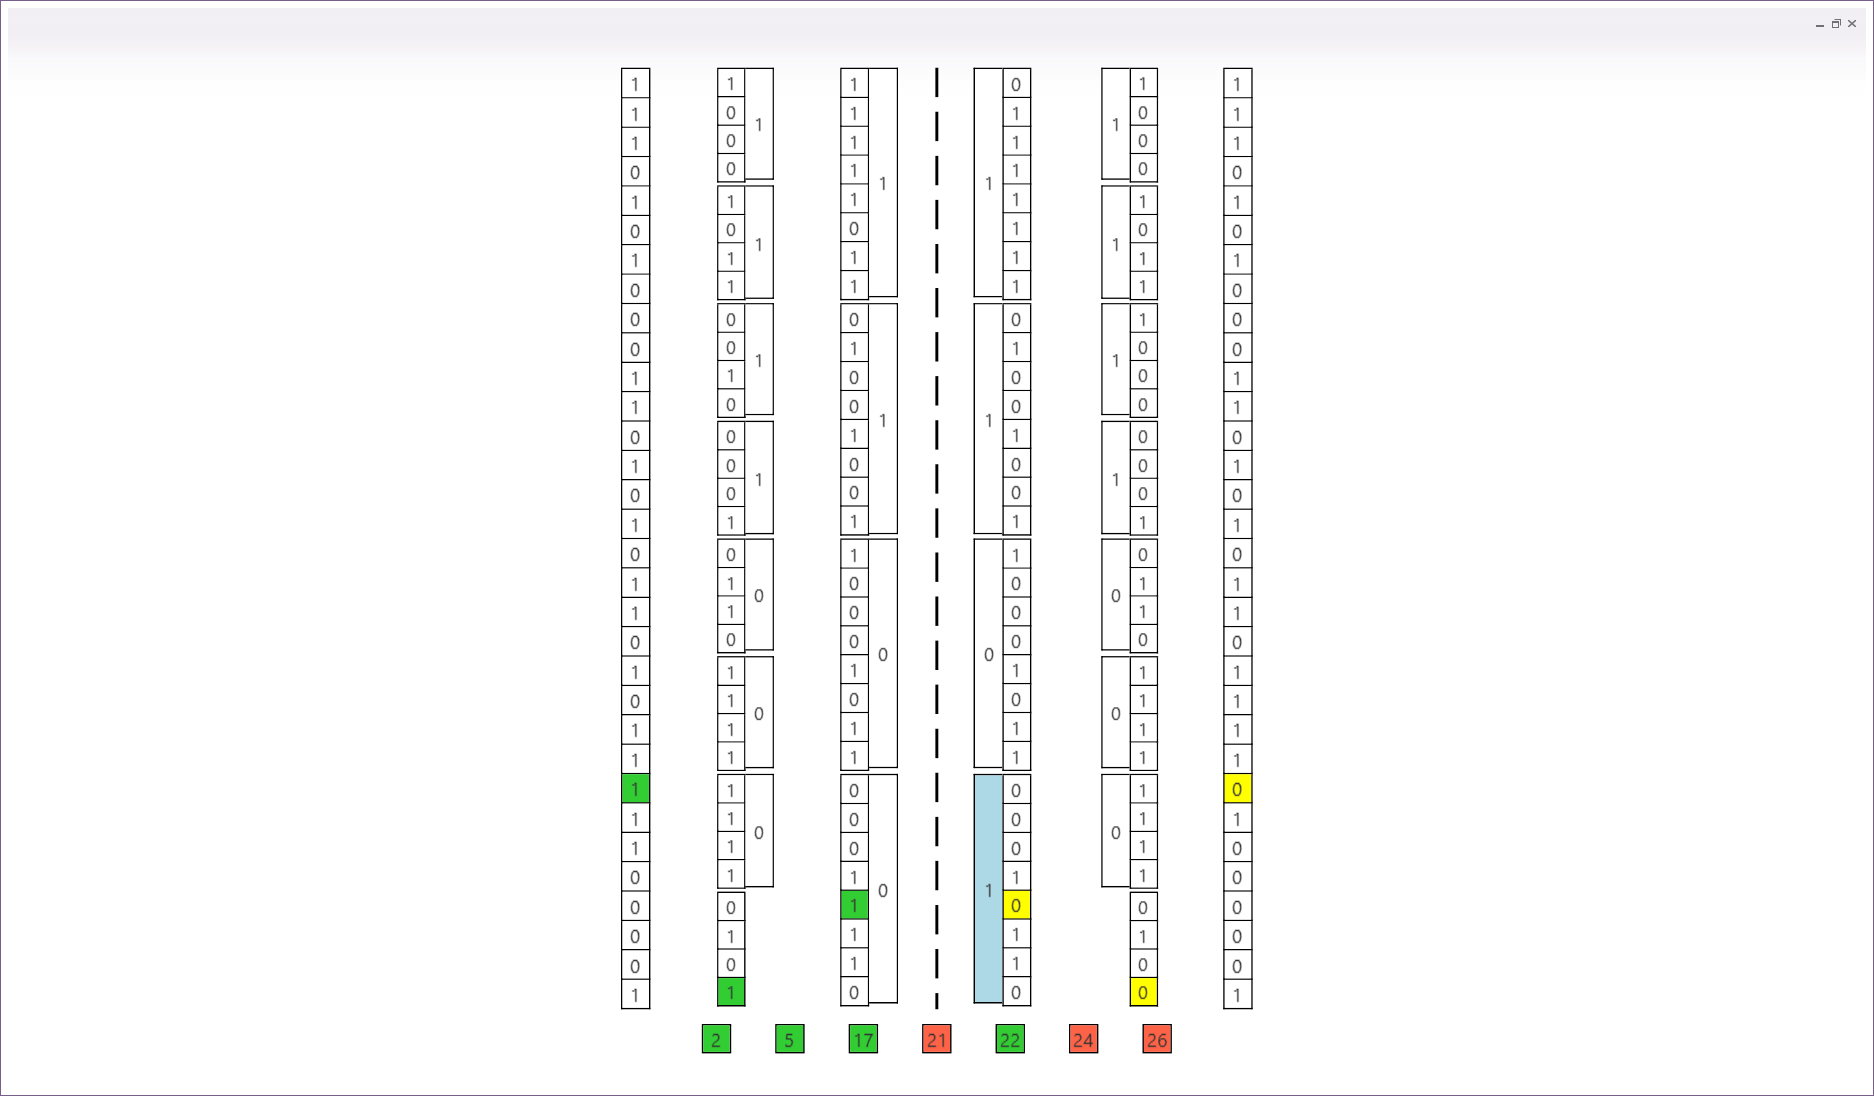
\includegraphics[width=1\linewidth]{chapter3/cascade_screenshots/15_error_found}}
   \only<17>{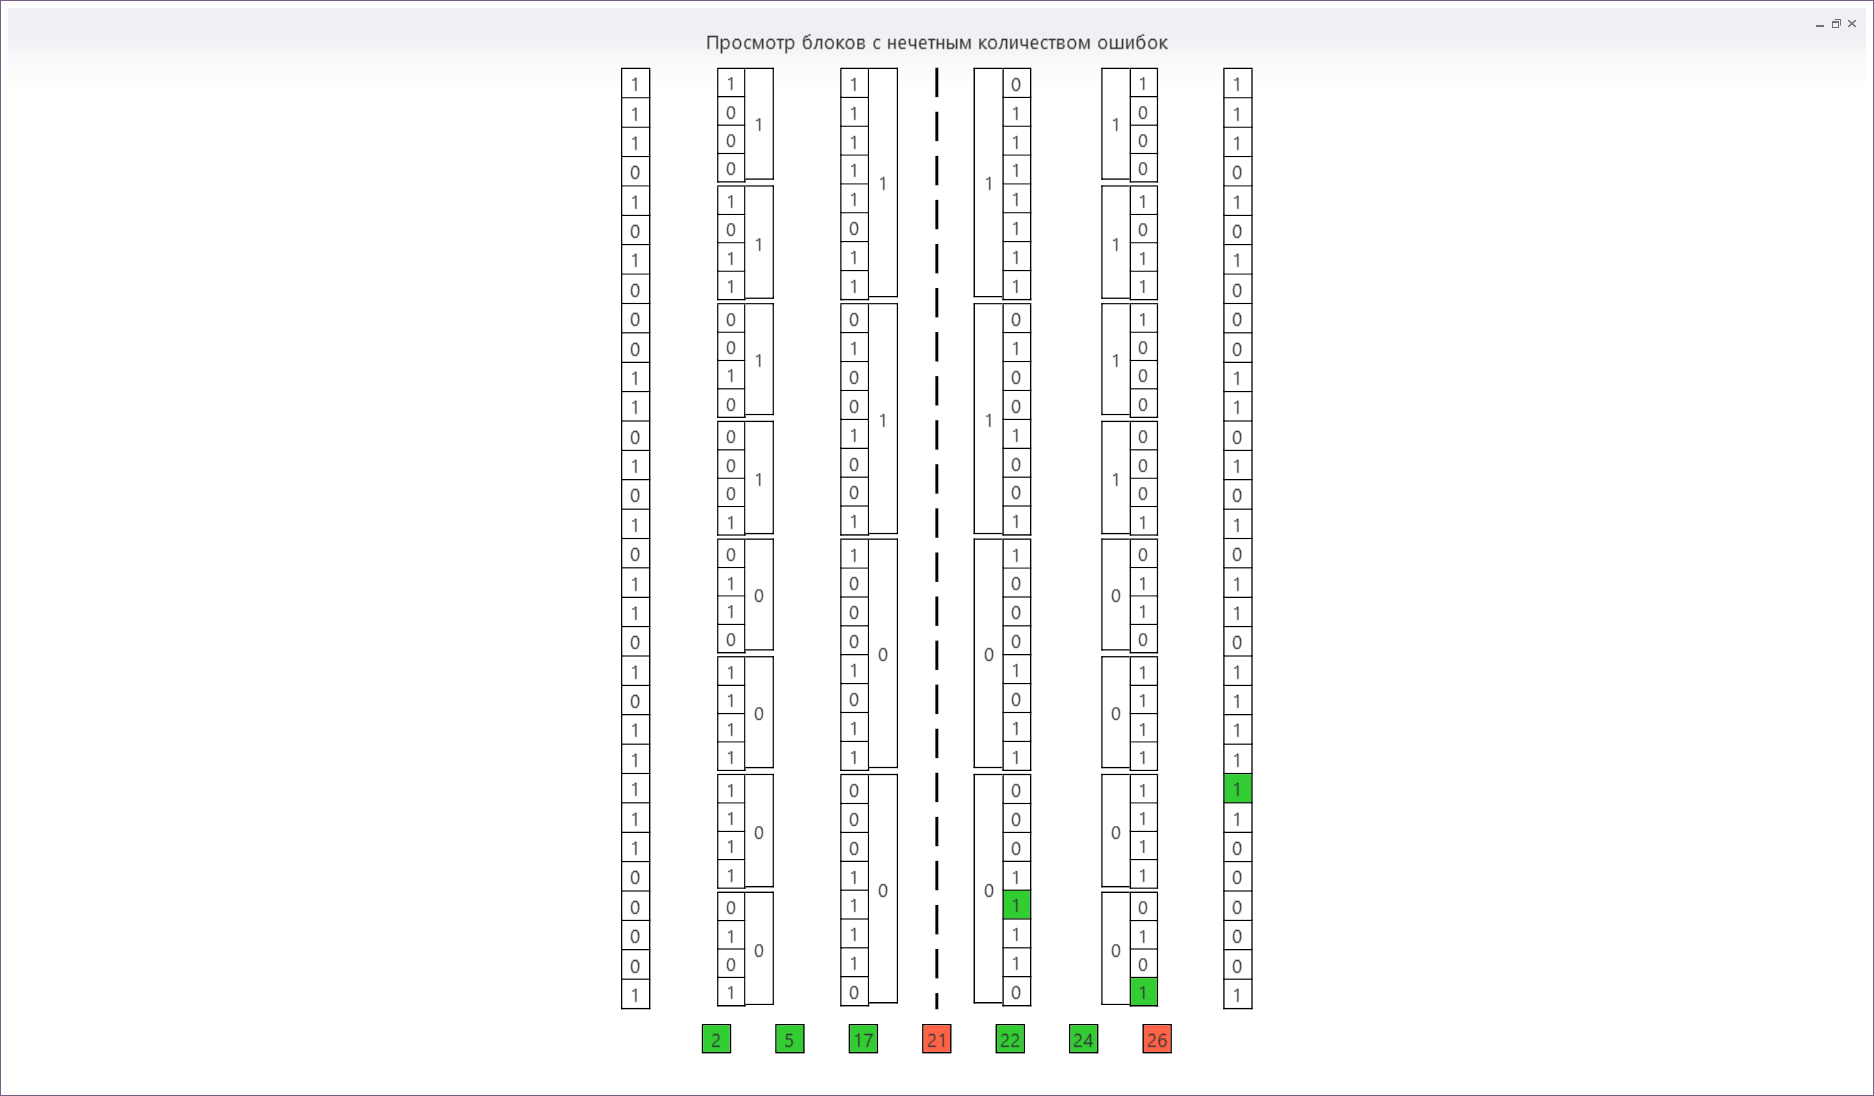
\includegraphics[width=1\linewidth]{chapter3/cascade_screenshots/16_error_backtrace}}
   \only<18>{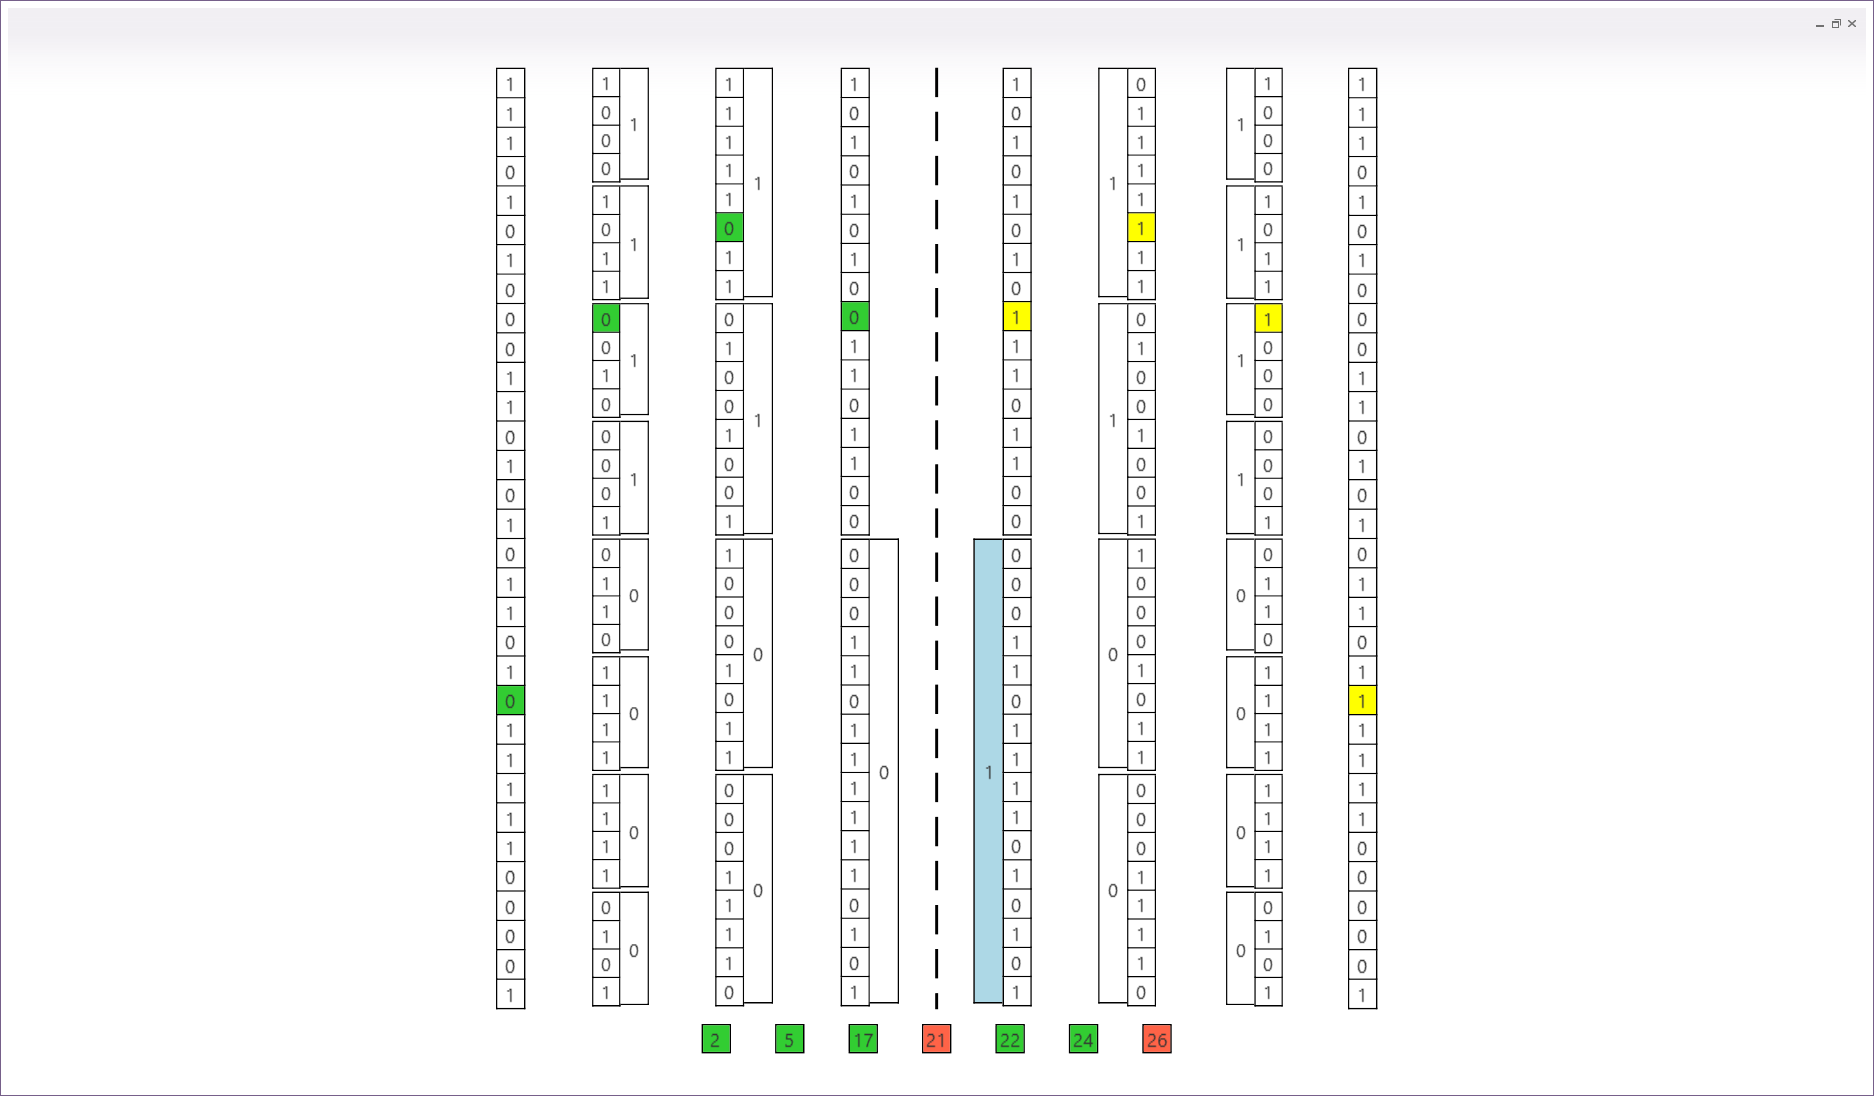
\includegraphics[width=1\linewidth]{chapter3/cascade_screenshots/17_error_found}}
   \only<19>{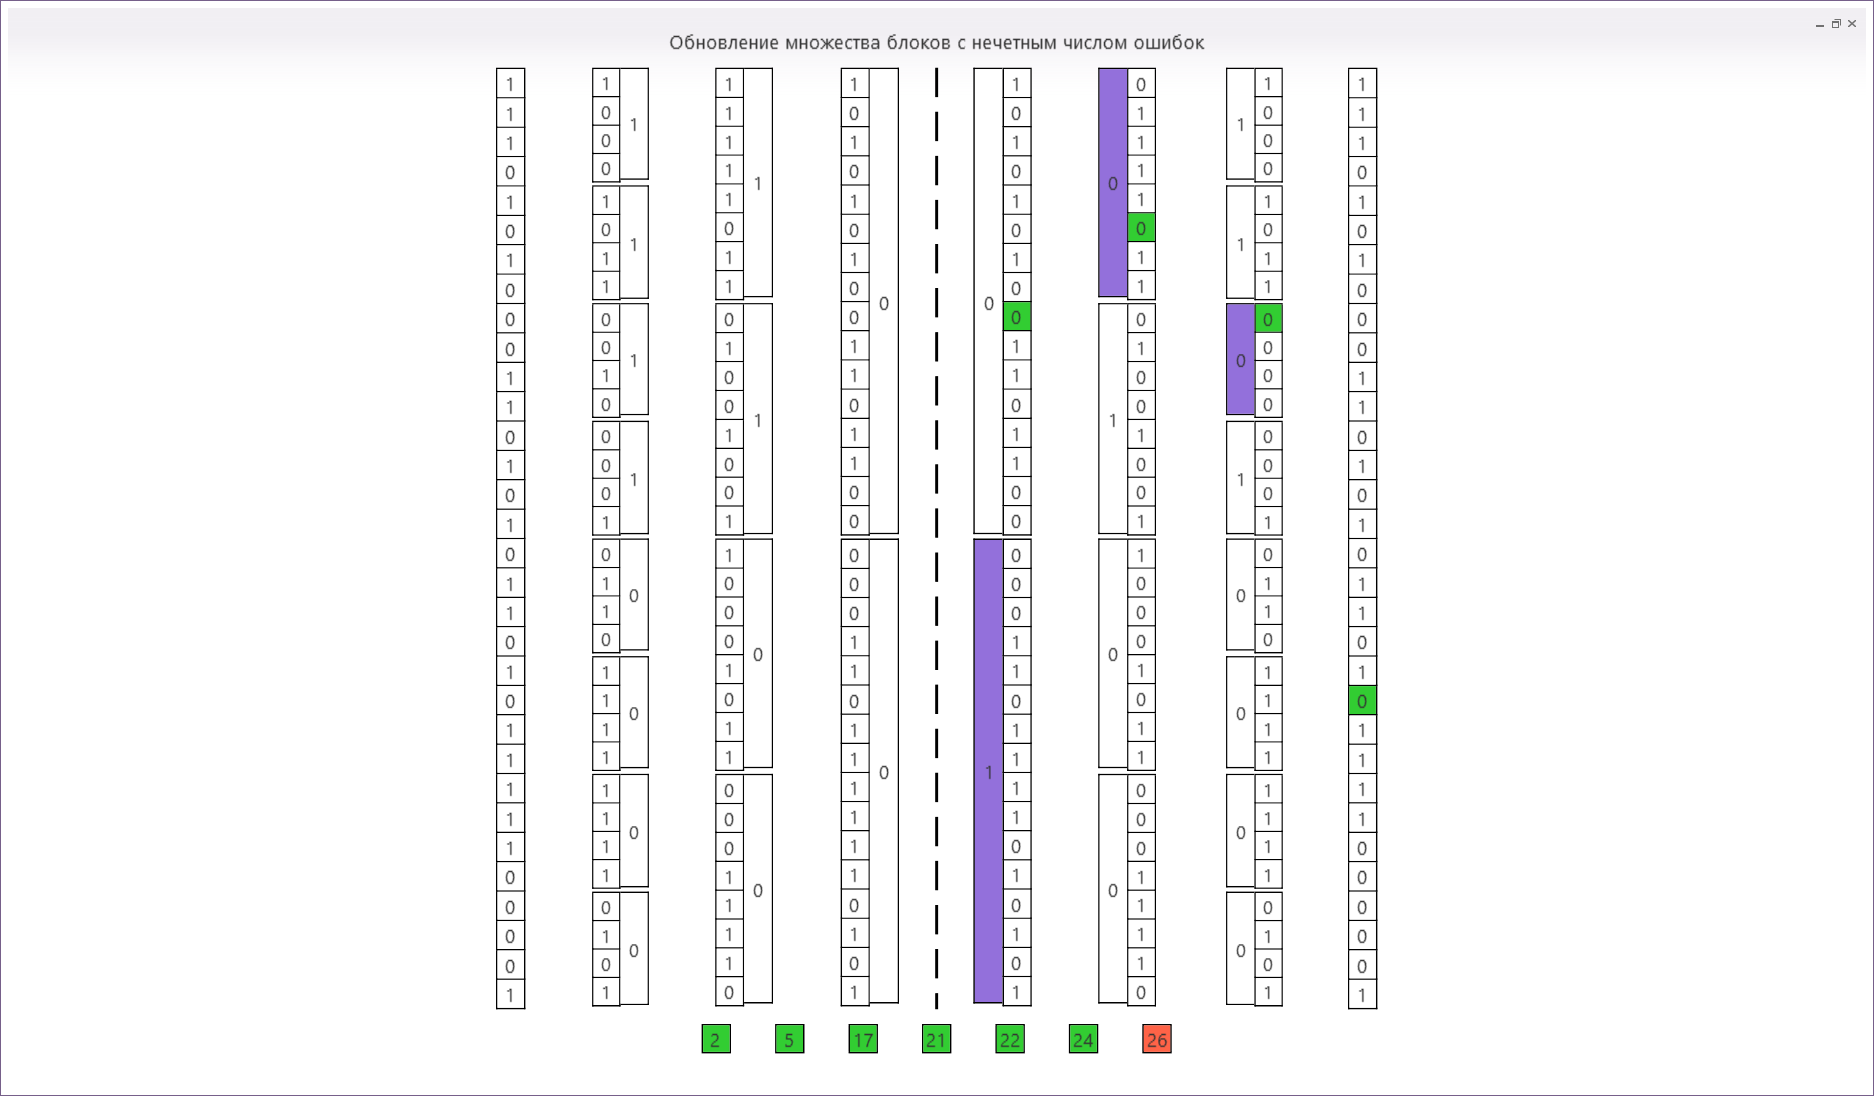
\includegraphics[width=1\linewidth]{chapter3/cascade_screenshots/18_error_backtrace}}
   \only<20>{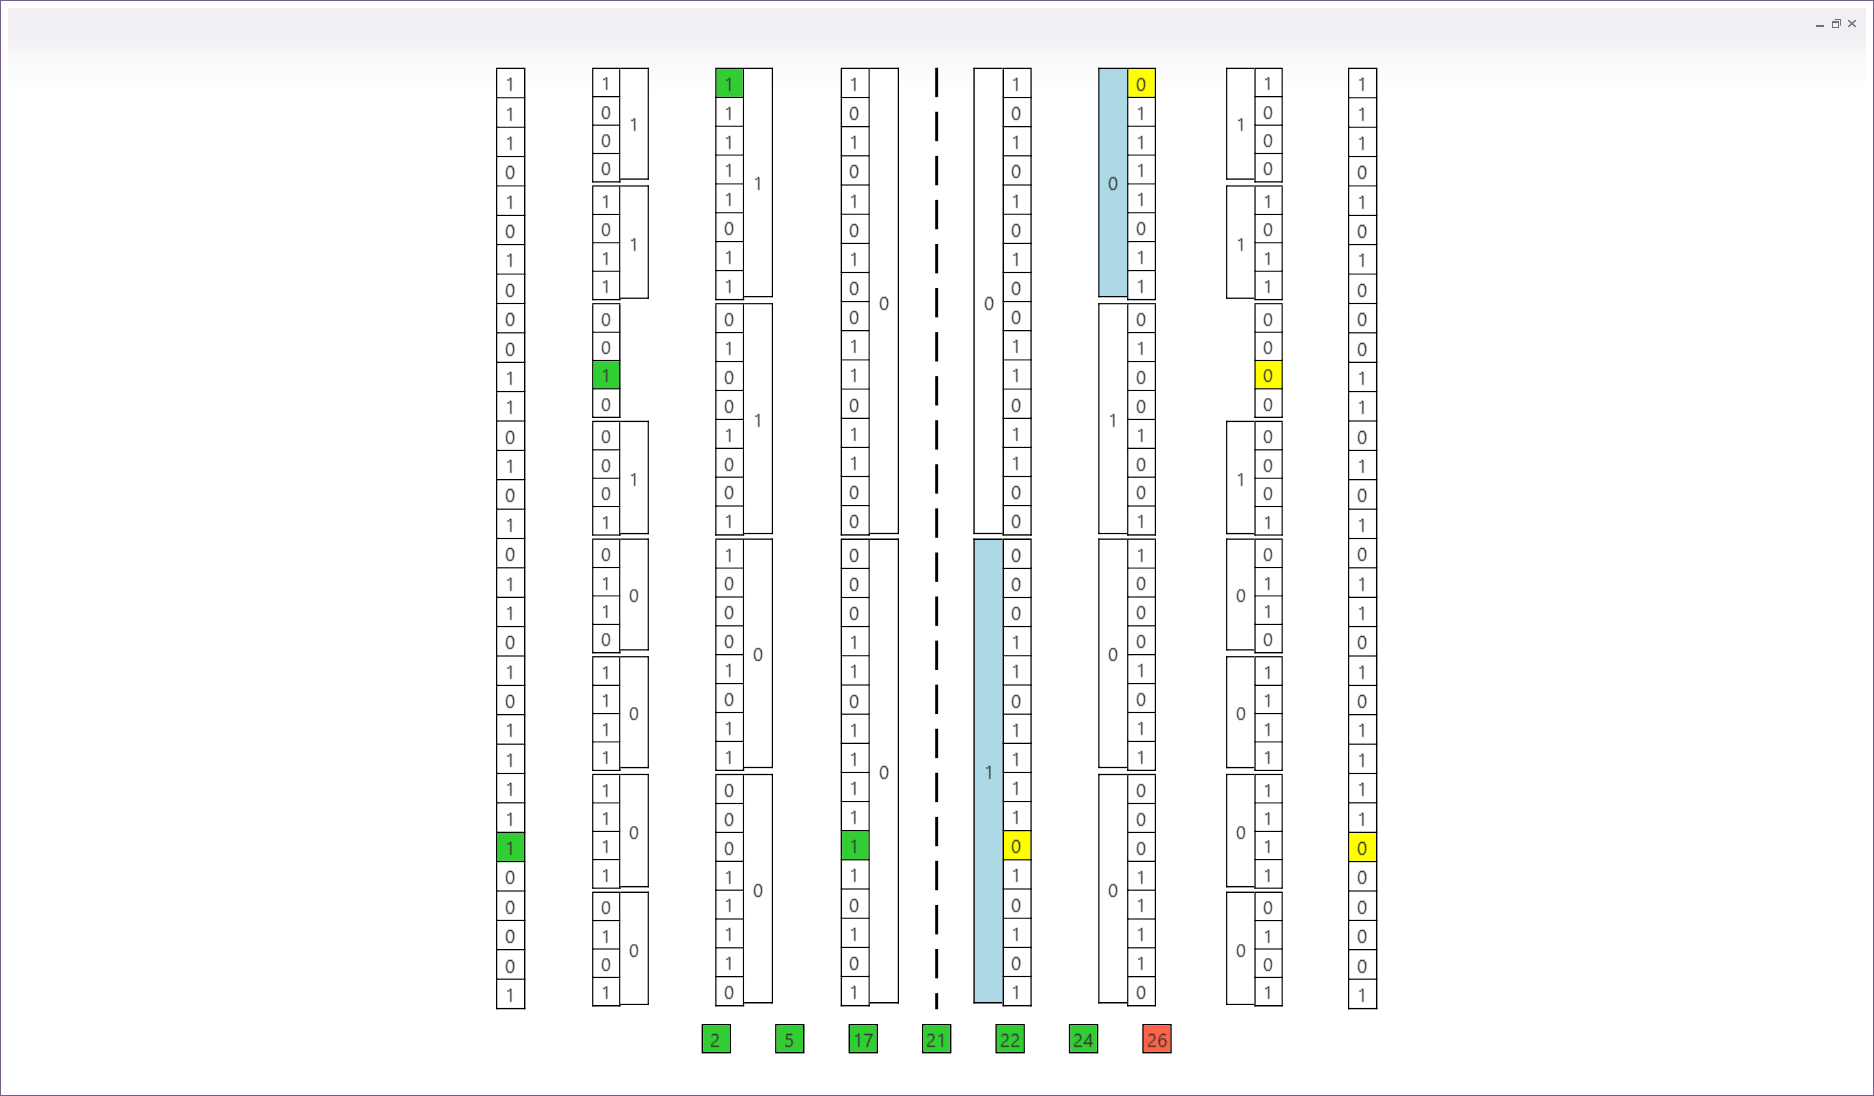
\includegraphics[width=1\linewidth]{chapter3/cascade_screenshots/19_error_found}}
   \only<21>{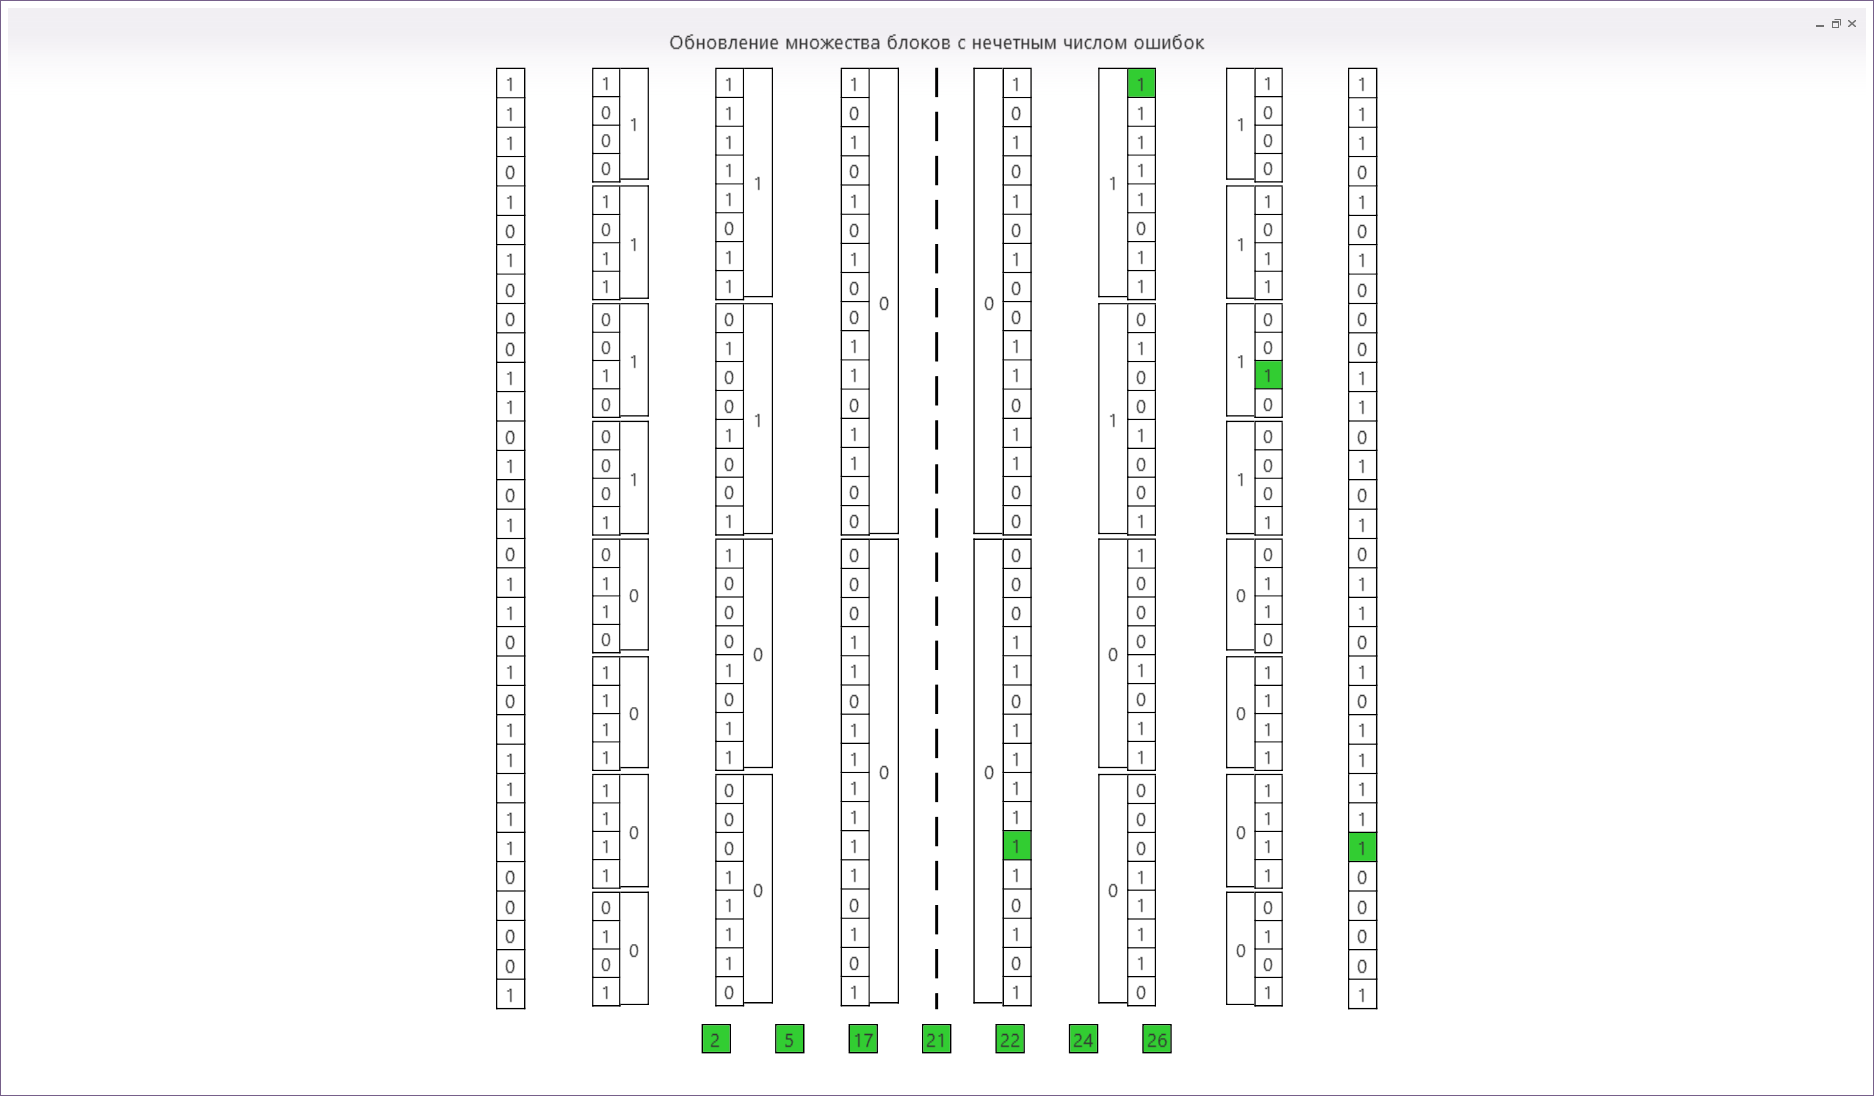
\includegraphics[width=1\linewidth]{chapter3/cascade_screenshots/20_error_backtrace}}
   \only<22>{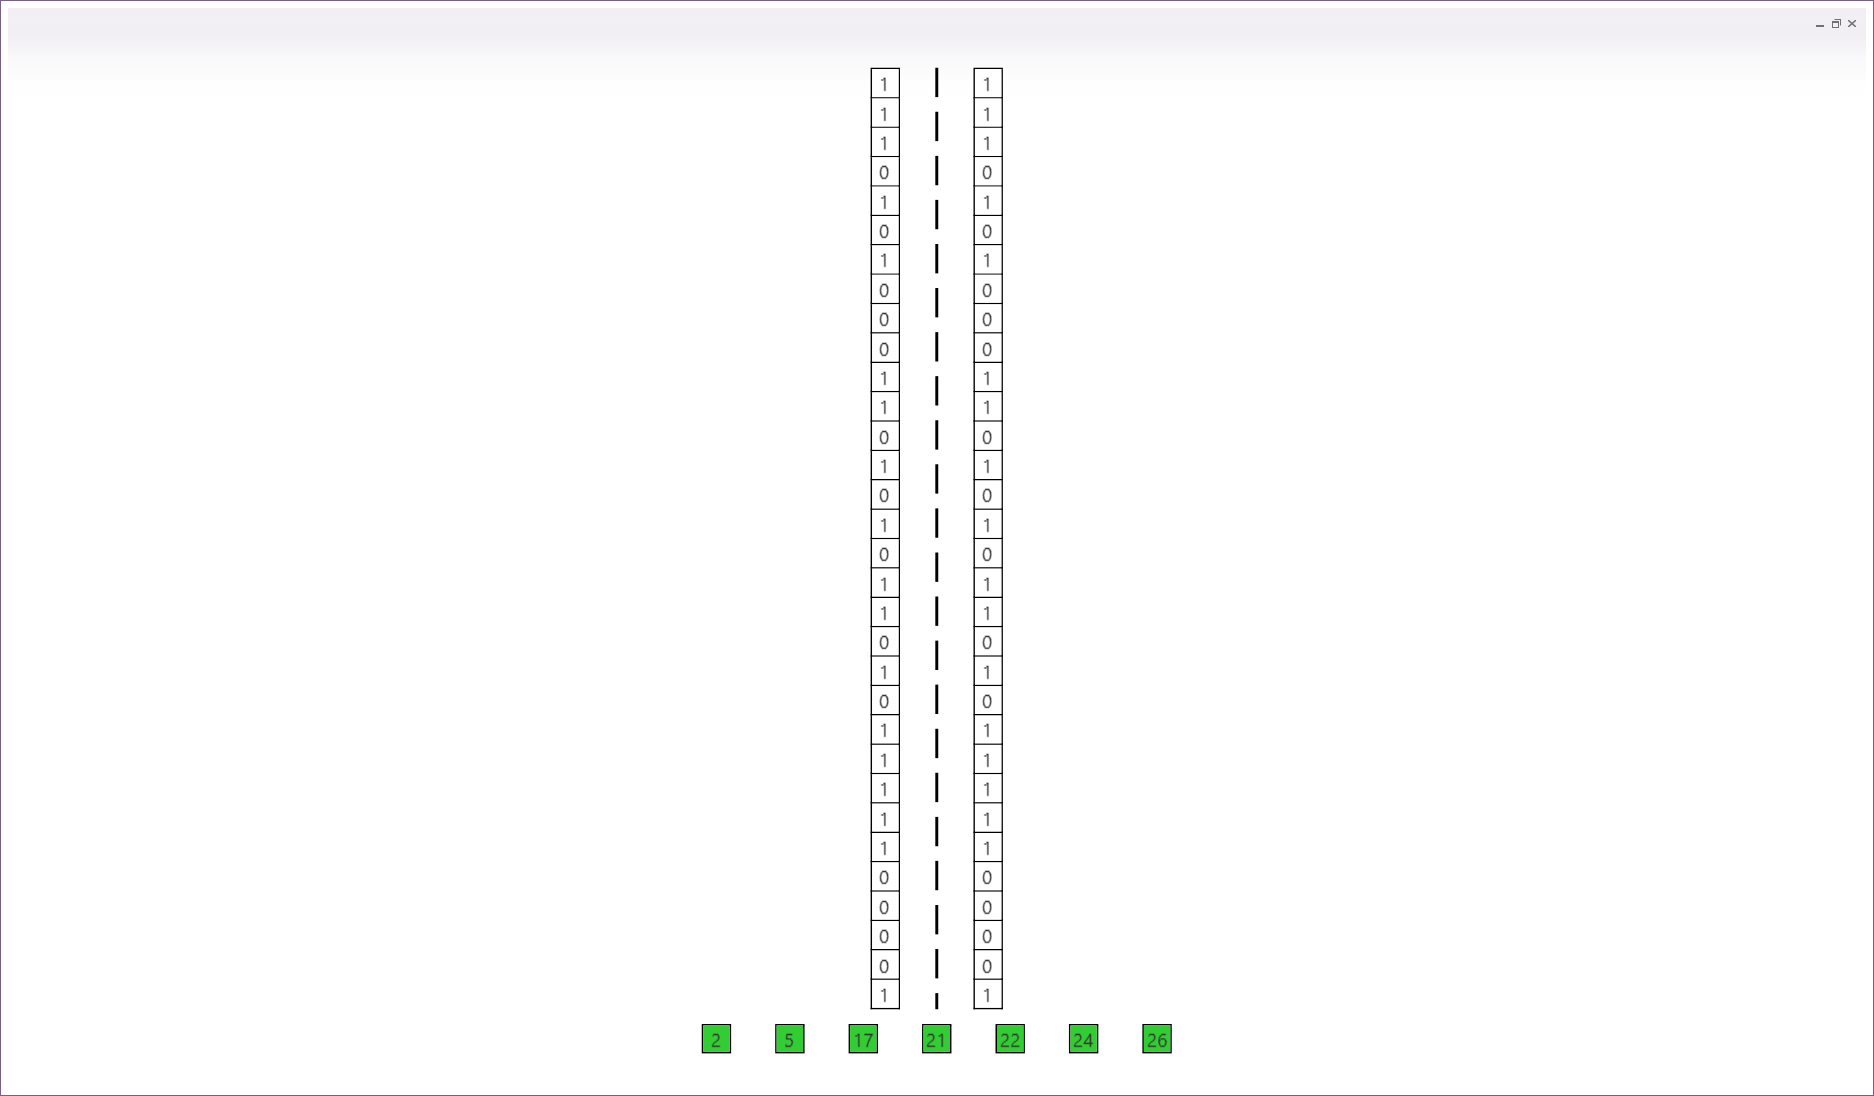
\includegraphics[width=1\linewidth]{chapter3/cascade_screenshots/21_end_state}}
 \end{frame}
 \note{ 
 Рассматриваемый каскадный протокол коррекции ошибок проходит в несколько шагов. Происходит разбитие ключа на несколько блоков, вычисляется некоторая характеристика каждого блока (например, четность), Алиса посылает свои четности, Боб сверяет со своими, и сообщает, в каких блоках четность не совпала. Эти блоки формируют множество блоков с нечетным числом ошибок, с которым происходит вся дальнейшая работа.}\note{
 До тех пор, пока это множество не пусто, из него выбирается один блок наименьшего размера, и производится дихотомический поиск ошибки, то есть сначала сравниваются четности первых половин соответствующих блоков. Если они совпадают, то ошибка кроется во второй половине, если различаются~--- в первой. Таким образом находится позиция, содержащая ошибку.}
 \note{Каскадным протокол называется из-за следующей схемы работы. Все блоки, которые на прошлых проходах содержали в себе только что исправленную позицию, вносятся в множество с нечетным числом ошибок. Если же они там уже были, то удаляются. Таким образом обнаружение ошибки в блоке третьего прохода вызовет каскадное обнаружение ошибки в блоках первого или второго прохода, что в свою очередь вызовет обнаружение ошибки в еще каком-либо блоке, и так до тех пор, пока множество блоков с нечетным числом ошибок не окажется пустым.
 }
 
 
 \begin{frame}{Сжатие полученного ключа}
 \only<1>{\begin{definition}
  Семейство $\mathcal{F}$ функций $\mathcal{A}\rightarrow\mathcal{B}$ называется \textit{универсальным}, если 
  $$  \pr[f(x_1) = f(x_2)] < \frac{1}{|\mathcal{B}|} ~~\forall x_1, x_2 \in \mathcal{A}: x_1 \neq x_2, $$ а $f$ выбирается из $\mathcal{F}$ в соответствии с равномерным распределением.
\end{definition}}
\only<2>{
   \begin{theorem}
  Пусть $X$~--- случайная величина в алфавите $\mathcal{X}$ с вероятностым распределением $P_X$ и энтропией Реньи $R(X)$. Кроме того, пусть $G$~--- случайная величина, отвечающая случайному выбору (внутри равномерного распределения) члена универсального семейства хеш-функций, отображающих $\mathcal{X} \rightarrow \{0,1\}^r$. Тогда
  \begin{equation}
    H(G(X)|G) \geq R(G(X)|G) \geq r - \frac{2^{r - R(X)}}{\ln 2}.
  \end{equation}
\end{theorem}
}
\end{frame}

 \note{ 
 После проведения процедуры коррекции ошибок Алисе и Бобу известно примерное количество информации, которое могло стать доступным Еве в ходе работы протокола распределения ключей и коррекции ошибок.
 Зная эту величину, они могут провести сжатие ключа путем хеширования функциями из универсального семейства хеш-функций, определение которых вы видите на слайде. Сама хеш функция выбирается случайным образом из заранее известного универсального семейства хеш-функций, то есть является случайной величиной. В результате Алиса и Боб получат ключ меньшей длины, но информация Евы о нем будет бесконечно малой. 
 В итоге цель достигнута: стороны имеют общий секретный ключ, о котором злоумышленник ничего не знает.
 }
 
 
\section{Описание практической реализации и полученных результатов}
 \begin{frame}{Полученные результаты}
   \begin{enumerate}
     \item Показано существование и дано обоснование секретности протокола квантовой криптографии, обеспечивающего безусловную секретность в условиях потерь в линии связи и неоднофотонности источника.
      \item Рассмотрен и проанализирован один из протоколов коррекции ошибок, который в настоящее время является стандартом в квантовом распределении ключей.
\item Разработаны программы, визуализирующие процессы:
\begin{itemize}
  \item распределения ключей по релятивистскому протоколу с имитацией атак подслушивателя и последующим детектированием возникающих из-за этого задержек,
  \item коррекции ошибок по протоколу Cascade.
\end{itemize}
   \end{enumerate}
 \end{frame}
 
 \note{
 Для моделирования и визуализации релятивистского протокола квантового распределения ключей и каскадного протокола коррекции ошибок было написано две программы.
 Обе написаны на языке C\#, требуют установленного .NET 4.5, используют шаблон проектирования MVVM, и богатые возможности платформы Windows Presentation Framework (WPF) по анимации контента.
 
 Снимки экрана программы коррекции ошибок были показаны ранее, а сейчас я хочу продемонстрировать основную разработку - визуализация релятивистского протокола, пока позволяет время.
}



\maketitle
\end{document}
